\documentclass{book}
\usepackage[a4paper,top=2.5cm,bottom=2.5cm,left=2.5cm,right=2.5cm]{geometry}
\usepackage{makeidx}
\usepackage{natbib}
\usepackage{graphicx}
\usepackage{multicol}
\usepackage{float}
\usepackage{listings}
\usepackage{color}
\usepackage{ifthen}
\usepackage[table]{xcolor}
\usepackage{textcomp}
\usepackage{alltt}
\usepackage{ifpdf}
\ifpdf
\usepackage[pdftex,
            pagebackref=true,
            colorlinks=true,
            linkcolor=blue,
            unicode
           ]{hyperref}
\else
\usepackage[ps2pdf,
            pagebackref=true,
            colorlinks=true,
            linkcolor=blue,
            unicode
           ]{hyperref}
\usepackage{pspicture}
\fi
\usepackage[utf8]{inputenc}
\usepackage{mathptmx}
\usepackage[scaled=.90]{helvet}
\usepackage{courier}
\usepackage{sectsty}
\usepackage{amssymb}
\usepackage[titles]{tocloft}
\usepackage{doxygen}
\lstset{language=C++,inputencoding=utf8,basicstyle=\footnotesize,breaklines=true,breakatwhitespace=true,tabsize=8,numbers=left }
\makeindex
\setcounter{tocdepth}{3}
\renewcommand{\footrulewidth}{0.4pt}
\renewcommand{\familydefault}{\sfdefault}
\hfuzz=15pt
\setlength{\emergencystretch}{15pt}
\hbadness=750
\tolerance=750
\begin{document}
\hypersetup{pageanchor=false,citecolor=blue}
\begin{titlepage}
\vspace*{7cm}
\begin{center}
{\Large X\-T\-D }\\
\vspace*{1cm}
{\large Generated by Doxygen 1.8.1.2}\\
\vspace*{0.5cm}
{\small Thu Aug 7 2014 15:49:58}\\
\end{center}
\end{titlepage}
\clearemptydoublepage
\pagenumbering{roman}
\tableofcontents
\clearemptydoublepage
\pagenumbering{arabic}
\hypersetup{pageanchor=true,citecolor=blue}
\chapter{Namespace Index}
\section{Namespace List}
Here is a list of all documented namespaces with brief descriptions\-:\begin{DoxyCompactList}
\item\contentsline{section}{\hyperlink{namespacestr}{str} \\*A namespace containing tools for operations which strings }{\pageref{namespacestr}}{}
\item\contentsline{section}{\hyperlink{namespacextd}{xtd} \\*A root namespace of the library }{\pageref{namespacextd}}{}
\end{DoxyCompactList}

\chapter{Class Index}
\section{Class Hierarchy}
This inheritance list is sorted roughly, but not completely, alphabetically\-:\begin{DoxyCompactList}
\item \contentsline{section}{xstd\-:\-:abstract\-\_\-functor$<$ arguments\-\_\-type $>$}{\pageref{classxstd_1_1abstract__functor}}{}
\item \contentsline{section}{xstd\-:\-:abstract\-\_\-functor$<$ arguments\-\_\-type...$>$}{\pageref{classxstd_1_1abstract__functor}}{}
\begin{DoxyCompactList}
\item \contentsline{section}{xstd\-:\-:functor$<$ object\-\_\-type, arguments\-\_\-type $>$}{\pageref{classxstd_1_1functor}}{}
\end{DoxyCompactList}
\item \contentsline{section}{xstd\-:\-:abstract\-\_\-logger}{\pageref{classxstd_1_1abstract__logger}}{}
\begin{DoxyCompactList}
\item \contentsline{section}{xstd\-:\-:console\-\_\-logger}{\pageref{classxstd_1_1console__logger}}{}
\item \contentsline{section}{xstd\-:\-:file\-\_\-logger}{\pageref{classxstd_1_1file__logger}}{}
\end{DoxyCompactList}
\item \contentsline{section}{xstd\-:\-:coutmt\-\_\-singleton}{\pageref{classxstd_1_1coutmt__singleton}}{}
\item \contentsline{section}{xstd\-:\-:dimension\-\_\-mismatch}{\pageref{structxstd_1_1dimension__mismatch}}{}
\item \contentsline{section}{xstd\-:\-:event$<$ data\-\_\-type $>$}{\pageref{classxstd_1_1event}}{}
\item \contentsline{section}{xstd\-:\-:pp\-:\-:first\-\_\-type$<$ parameters\-\_\-types $>$}{\pageref{structxstd_1_1pp_1_1first__type}}{}
\item \contentsline{section}{xstd\-:\-:pp\-:\-:is\-\_\-heterogeneous$<$ parameters\-\_\-types $>$}{\pageref{structxstd_1_1pp_1_1is__heterogeneous}}{}
\item \contentsline{section}{xstd\-:\-:pp\-:\-:is\-\_\-homogeneous$<$ parameters\-\_\-types $>$}{\pageref{structxstd_1_1pp_1_1is__homogeneous}}{}
\item \contentsline{section}{xstd\-:\-:pp\-:\-:is\-\_\-homogeneous$<$ first\-\_\-parameter\-\_\-type, other\-\_\-parameters\-\_\-types... $>$}{\pageref{structxstd_1_1pp_1_1is__homogeneous_3_01first__parameter__type_00_01other__parameters__types_8_8_8_01_4}}{}
\item \contentsline{section}{xstd\-:\-:pp\-:\-:is\-\_\-homogeneous$<$ parameter\-\_\-type $>$}{\pageref{structxstd_1_1pp_1_1is__homogeneous_3_01parameter__type_01_4}}{}
\item \contentsline{section}{xstd\-:\-:pp\-:\-:last\-\_\-type$<$ parameters\-\_\-types $>$}{\pageref{structxstd_1_1pp_1_1last__type}}{}
\item \contentsline{section}{xstd\-:\-:logger\-\_\-client}{\pageref{classxstd_1_1logger__client}}{}
\item \contentsline{section}{xstd\-:\-:pp\-:\-:nth\-\_\-type$<$ parameter\-\_\-id, parameters\-\_\-types $>$}{\pageref{structxstd_1_1pp_1_1nth__type}}{}
\item \contentsline{section}{xstd\-:\-:pp\-:\-:nth\-\_\-type\-\_\-helper$<$ parameter\-\_\-id, parameters\-\_\-types $>$}{\pageref{structxstd_1_1pp_1_1nth__type__helper}}{}
\item \contentsline{section}{xstd\-:\-:pp\-:\-:nth\-\_\-type\-\_\-helper$<$ 0, first\-\_\-parameter\-\_\-type, other\-\_\-parameters\-\_\-types... $>$}{\pageref{structxstd_1_1pp_1_1nth__type__helper_3_010_00_01first__parameter__type_00_01other__parameters__types_8_8_8_01_4}}{}
\item \contentsline{section}{xstd\-:\-:pp\-:\-:nth\-\_\-type\-\_\-helper$<$ parameter\-\_\-id, first\-\_\-parameter\-\_\-type, other\-\_\-parameters\-\_\-types... $>$}{\pageref{structxstd_1_1pp_1_1nth__type__helper_3_01parameter__id_00_01first__parameter__type_00_01other__parameters__types_8_8_8_01_4}}{}
\item \contentsline{section}{xstd\-:\-:pp\-:\-:null\-\_\-type}{\pageref{structxstd_1_1pp_1_1null__type}}{}
\item \contentsline{section}{xstd\-:\-:point$<$ type, dimension $>$}{\pageref{classxstd_1_1point}}{}
\item \contentsline{section}{printer}{\pageref{structprinter}}{}
\item \contentsline{section}{xstd\-:\-:raii\-\_\-thread\-\_\-base}{\pageref{classxstd_1_1raii__thread__base}}{}
\begin{DoxyCompactList}
\item \contentsline{section}{xstd\-:\-:raii\-\_\-thread}{\pageref{classxstd_1_1raii__thread}}{}
\item \contentsline{section}{xstd\-:\-:raii\-\_\-thread\-\_\-manual}{\pageref{classxstd_1_1raii__thread__manual}}{}
\end{DoxyCompactList}
\item \contentsline{section}{xstd\-:\-:chrono\-:\-:timer\-\_\-base}{\pageref{classxstd_1_1chrono_1_1timer__base}}{}
\begin{DoxyCompactList}
\item \contentsline{section}{xstd\-:\-:chrono\-:\-:timer$<$ clock $>$}{\pageref{classxstd_1_1chrono_1_1timer}}{}
\end{DoxyCompactList}
\item \contentsline{section}{xstd\-:\-:chrono\-:\-:timer\-\_\-manager}{\pageref{classxstd_1_1chrono_1_1timer__manager}}{}
\end{DoxyCompactList}

\chapter{Class Index}
\section{Class List}
Here are the classes, structs, unions and interfaces with brief descriptions\-:\begin{DoxyCompactList}
\item\contentsline{section}{\hyperlink{classxstd_1_1abstract__functor}{xstd\-::abstract\-\_\-functor$<$ arguments\-\_\-type $>$} }{\pageref{classxstd_1_1abstract__functor}}{}
\item\contentsline{section}{\hyperlink{classxstd_1_1abstract__logger}{xstd\-::abstract\-\_\-logger} }{\pageref{classxstd_1_1abstract__logger}}{}
\item\contentsline{section}{\hyperlink{classxstd_1_1console__logger}{xstd\-::console\-\_\-logger} }{\pageref{classxstd_1_1console__logger}}{}
\item\contentsline{section}{\hyperlink{classxstd_1_1coutmt__singleton}{xstd\-::coutmt\-\_\-singleton} }{\pageref{classxstd_1_1coutmt__singleton}}{}
\item\contentsline{section}{\hyperlink{structxstd_1_1dimension__mismatch}{xstd\-::dimension\-\_\-mismatch} }{\pageref{structxstd_1_1dimension__mismatch}}{}
\item\contentsline{section}{\hyperlink{classxstd_1_1event}{xstd\-::event$<$ data\-\_\-type $>$} }{\pageref{classxstd_1_1event}}{}
\item\contentsline{section}{\hyperlink{classxstd_1_1file__logger}{xstd\-::file\-\_\-logger} }{\pageref{classxstd_1_1file__logger}}{}
\item\contentsline{section}{\hyperlink{structxstd_1_1pp_1_1first__type}{xstd\-::pp\-::first\-\_\-type$<$ parameters\-\_\-types $>$} }{\pageref{structxstd_1_1pp_1_1first__type}}{}
\item\contentsline{section}{\hyperlink{classxstd_1_1functor}{xstd\-::functor$<$ object\-\_\-type, arguments\-\_\-type $>$} }{\pageref{classxstd_1_1functor}}{}
\item\contentsline{section}{\hyperlink{structxstd_1_1pp_1_1is__heterogeneous}{xstd\-::pp\-::is\-\_\-heterogeneous$<$ parameters\-\_\-types $>$} }{\pageref{structxstd_1_1pp_1_1is__heterogeneous}}{}
\item\contentsline{section}{\hyperlink{structxstd_1_1pp_1_1is__homogeneous}{xstd\-::pp\-::is\-\_\-homogeneous$<$ parameters\-\_\-types $>$} }{\pageref{structxstd_1_1pp_1_1is__homogeneous}}{}
\item\contentsline{section}{\hyperlink{structxstd_1_1pp_1_1is__homogeneous_3_01first__parameter__type_00_01other__parameters__types_8_8_8_01_4}{xstd\-::pp\-::is\-\_\-homogeneous$<$ first\-\_\-parameter\-\_\-type, other\-\_\-parameters\-\_\-types... $>$} }{\pageref{structxstd_1_1pp_1_1is__homogeneous_3_01first__parameter__type_00_01other__parameters__types_8_8_8_01_4}}{}
\item\contentsline{section}{\hyperlink{structxstd_1_1pp_1_1is__homogeneous_3_01parameter__type_01_4}{xstd\-::pp\-::is\-\_\-homogeneous$<$ parameter\-\_\-type $>$} }{\pageref{structxstd_1_1pp_1_1is__homogeneous_3_01parameter__type_01_4}}{}
\item\contentsline{section}{\hyperlink{structxstd_1_1pp_1_1last__type}{xstd\-::pp\-::last\-\_\-type$<$ parameters\-\_\-types $>$} }{\pageref{structxstd_1_1pp_1_1last__type}}{}
\item\contentsline{section}{\hyperlink{classxstd_1_1logger__client}{xstd\-::logger\-\_\-client} }{\pageref{classxstd_1_1logger__client}}{}
\item\contentsline{section}{\hyperlink{structxstd_1_1pp_1_1nth__type}{xstd\-::pp\-::nth\-\_\-type$<$ parameter\-\_\-id, parameters\-\_\-types $>$} }{\pageref{structxstd_1_1pp_1_1nth__type}}{}
\item\contentsline{section}{\hyperlink{structxstd_1_1pp_1_1nth__type__helper}{xstd\-::pp\-::nth\-\_\-type\-\_\-helper$<$ parameter\-\_\-id, parameters\-\_\-types $>$} }{\pageref{structxstd_1_1pp_1_1nth__type__helper}}{}
\item\contentsline{section}{\hyperlink{structxstd_1_1pp_1_1nth__type__helper_3_010_00_01first__parameter__type_00_01other__parameters__types_8_8_8_01_4}{xstd\-::pp\-::nth\-\_\-type\-\_\-helper$<$ 0, first\-\_\-parameter\-\_\-type, other\-\_\-parameters\-\_\-types... $>$} }{\pageref{structxstd_1_1pp_1_1nth__type__helper_3_010_00_01first__parameter__type_00_01other__parameters__types_8_8_8_01_4}}{}
\item\contentsline{section}{\hyperlink{structxstd_1_1pp_1_1nth__type__helper_3_01parameter__id_00_01first__parameter__type_00_01other__parameters__types_8_8_8_01_4}{xstd\-::pp\-::nth\-\_\-type\-\_\-helper$<$ parameter\-\_\-id, first\-\_\-parameter\-\_\-type, other\-\_\-parameters\-\_\-types... $>$} }{\pageref{structxstd_1_1pp_1_1nth__type__helper_3_01parameter__id_00_01first__parameter__type_00_01other__parameters__types_8_8_8_01_4}}{}
\item\contentsline{section}{\hyperlink{structxstd_1_1pp_1_1null__type}{xstd\-::pp\-::null\-\_\-type} }{\pageref{structxstd_1_1pp_1_1null__type}}{}
\item\contentsline{section}{\hyperlink{classxstd_1_1point}{xstd\-::point$<$ type, dimension $>$} }{\pageref{classxstd_1_1point}}{}
\item\contentsline{section}{\hyperlink{structprinter}{printer} }{\pageref{structprinter}}{}
\item\contentsline{section}{\hyperlink{classxstd_1_1raii__thread}{xstd\-::raii\-\_\-thread} }{\pageref{classxstd_1_1raii__thread}}{}
\item\contentsline{section}{\hyperlink{classxstd_1_1raii__thread__base}{xstd\-::raii\-\_\-thread\-\_\-base} }{\pageref{classxstd_1_1raii__thread__base}}{}
\item\contentsline{section}{\hyperlink{classxstd_1_1raii__thread__manual}{xstd\-::raii\-\_\-thread\-\_\-manual} }{\pageref{classxstd_1_1raii__thread__manual}}{}
\item\contentsline{section}{\hyperlink{classxstd_1_1chrono_1_1timer}{xstd\-::chrono\-::timer$<$ clock $>$} }{\pageref{classxstd_1_1chrono_1_1timer}}{}
\item\contentsline{section}{\hyperlink{classxstd_1_1chrono_1_1timer__base}{xstd\-::chrono\-::timer\-\_\-base} }{\pageref{classxstd_1_1chrono_1_1timer__base}}{}
\item\contentsline{section}{\hyperlink{classxstd_1_1chrono_1_1timer__manager}{xstd\-::chrono\-::timer\-\_\-manager} }{\pageref{classxstd_1_1chrono_1_1timer__manager}}{}
\end{DoxyCompactList}

\chapter{File Index}
\section{File List}
Here is a list of all documented files with brief descriptions\-:\begin{DoxyCompactList}
\item\contentsline{section}{src/chrono/chrono\-\_\-util/src/{\bfseries chrono\-\_\-util.\-hpp} }{\pageref{chrono__util_8hpp}}{}
\item\contentsline{section}{src/chrono/timer/timer/src/{\bfseries timer.\-hpp} }{\pageref{timer_8hpp}}{}
\item\contentsline{section}{src/chrono/timer/timer\-\_\-base/src/{\bfseries timer\-\_\-base.\-hpp} }{\pageref{timer__base_8hpp}}{}
\item\contentsline{section}{src/chrono/timer/timer\-\_\-manager/src/{\bfseries timer\-\_\-manager.\-hpp} }{\pageref{timer__manager_8hpp}}{}
\item\contentsline{section}{src/cmath/point/src/{\bfseries point.\-hpp} }{\pageref{point_8hpp}}{}
\item\contentsline{section}{src/cmath/random/src/{\bfseries random.\-hpp} }{\pageref{random_8hpp}}{}
\item\contentsline{section}{src/event/event/src/{\bfseries event.\-hpp} }{\pageref{event_8hpp}}{}
\item\contentsline{section}{src/fs/file\-\_\-util/src/{\bfseries file\-\_\-util.\-hpp} }{\pageref{file__util_8hpp}}{}
\item\contentsline{section}{src/functional/functor/abstract\-\_\-functor/src/{\bfseries abstract\-\_\-functor.\-hpp} }{\pageref{abstract__functor_8hpp}}{}
\item\contentsline{section}{src/functional/functor/functor/src/{\bfseries functor.\-hpp} }{\pageref{functor_8hpp}}{}
\item\contentsline{section}{src/iostream/coutmt/src/{\bfseries coutmt.\-hpp} }{\pageref{coutmt_8hpp}}{}
\item\contentsline{section}{src/log/abstract\-\_\-logger/src/{\bfseries abstract\-\_\-logger.\-hpp} }{\pageref{abstract__logger_8hpp}}{}
\item\contentsline{section}{src/log/console\-\_\-logger/src/{\bfseries console\-\_\-logger.\-hpp} }{\pageref{console__logger_8hpp}}{}
\item\contentsline{section}{src/log/file\-\_\-logger/src/{\bfseries file\-\_\-logger.\-hpp} }{\pageref{file__logger_8hpp}}{}
\item\contentsline{section}{src/log/logger\-\_\-client/src/{\bfseries logger\-\_\-client.\-hpp} }{\pageref{logger__client_8hpp}}{}
\item\contentsline{section}{src/memory/memory\-\_\-util/src/{\bfseries memory\-\_\-util.\-hpp} }{\pageref{memory__util_8hpp}}{}
\item\contentsline{section}{src/string/string\-\_\-util/src/\hyperlink{string__util_8hpp}{string\-\_\-util.\-hpp} }{\pageref{string__util_8hpp}}{}
\item\contentsline{section}{src/thread/raii\-\_\-thread/src/{\bfseries raii\-\_\-thread.\-hpp} }{\pageref{raii__thread_8hpp}}{}
\item\contentsline{section}{src/thread/raii\-\_\-thread\-\_\-base/src/{\bfseries raii\-\_\-thread\-\_\-base.\-hpp} }{\pageref{raii__thread__base_8hpp}}{}
\item\contentsline{section}{src/thread/raii\-\_\-thread\-\_\-manual/src/{\bfseries raii\-\_\-thread\-\_\-manual.\-hpp} }{\pageref{raii__thread__manual_8hpp}}{}
\item\contentsline{section}{src/utility/parameter\-\_\-pack/parameter\-\_\-pack\-\_\-element\-\_\-type/src/{\bfseries parameter\-\_\-pack\-\_\-element\-\_\-type.\-hpp} }{\pageref{parameter__pack__element__type_8hpp}}{}
\item\contentsline{section}{src/utility/parameter\-\_\-pack/parameter\-\_\-pack\-\_\-element\-\_\-value/src/{\bfseries parameter\-\_\-pack\-\_\-element\-\_\-value.\-hpp} }{\pageref{parameter__pack__element__value_8hpp}}{}
\item\contentsline{section}{src/utility/parameter\-\_\-pack/parameter\-\_\-pack\-\_\-for\-\_\-each/src/{\bfseries parameter\-\_\-pack\-\_\-for\-\_\-each.\-hpp} }{\pageref{parameter__pack__for__each_8hpp}}{}
\item\contentsline{section}{src/utility/parameter\-\_\-pack/parameter\-\_\-pack\-\_\-homogeneity/src/{\bfseries parameter\-\_\-pack\-\_\-homogeneity.\-hpp} }{\pageref{parameter__pack__homogeneity_8hpp}}{}
\end{DoxyCompactList}

\chapter{Namespace Documentation}
\hypertarget{namespacestr}{\section{str Namespace Reference}
\label{namespacestr}\index{str@{str}}
}


A namespace containing tools for operations which strings.  




\subsection{Detailed Description}
A namespace containing tools for operations which strings. 
\hypertarget{namespacextd}{\section{xtd Namespace Reference}
\label{namespacextd}\index{xtd@{xtd}}
}


A root namespace of the library.  




\subsection{Detailed Description}
A root namespace of the library. 
\chapter{Class Documentation}
\hypertarget{classxstd_1_1abstract__functor}{\section{xstd\-:\-:abstract\-\_\-functor$<$ arguments\-\_\-type $>$ Class Template Reference}
\label{classxstd_1_1abstract__functor}\index{xstd\-::abstract\-\_\-functor$<$ arguments\-\_\-type $>$@{xstd\-::abstract\-\_\-functor$<$ arguments\-\_\-type $>$}}
}


{\ttfamily \#include $<$abstract\-\_\-functor.\-hpp$>$}

\subsection*{Public Member Functions}
\begin{DoxyCompactItemize}
\item 
virtual \hyperlink{classxstd_1_1abstract__functor_a9f6e6b78fe73cc12ef0c2fc1b28cd8fd}{$\sim$abstract\-\_\-functor} (void)
\item 
virtual void \hyperlink{classxstd_1_1abstract__functor_aa396ab9aba29660208608903e1703359}{operator()} (arguments\-\_\-type...\-arguments) const =0
\item 
virtual void \hyperlink{classxstd_1_1abstract__functor_ae729729f945ed0d871768fc99e76d228}{invoke} (arguments\-\_\-type...\-arguments) const =0
\end{DoxyCompactItemize}


\subsection{Constructor \& Destructor Documentation}
\hypertarget{classxstd_1_1abstract__functor_a9f6e6b78fe73cc12ef0c2fc1b28cd8fd}{\index{xstd\-::abstract\-\_\-functor@{xstd\-::abstract\-\_\-functor}!$\sim$abstract\-\_\-functor@{$\sim$abstract\-\_\-functor}}
\index{$\sim$abstract\-\_\-functor@{$\sim$abstract\-\_\-functor}!xstd::abstract_functor@{xstd\-::abstract\-\_\-functor}}
\subsubsection[{$\sim$abstract\-\_\-functor}]{\setlength{\rightskip}{0pt plus 5cm}template$<$typename... arguments\-\_\-type$>$ virtual {\bf xstd\-::abstract\-\_\-functor}$<$ arguments\-\_\-type $>$\-::$\sim${\bf abstract\-\_\-functor} (
\begin{DoxyParamCaption}
\item[{void}]{}
\end{DoxyParamCaption}
)\hspace{0.3cm}{\ttfamily [virtual]}}}\label{classxstd_1_1abstract__functor_a9f6e6b78fe73cc12ef0c2fc1b28cd8fd}


\subsection{Member Function Documentation}
\hypertarget{classxstd_1_1abstract__functor_ae729729f945ed0d871768fc99e76d228}{\index{xstd\-::abstract\-\_\-functor@{xstd\-::abstract\-\_\-functor}!invoke@{invoke}}
\index{invoke@{invoke}!xstd::abstract_functor@{xstd\-::abstract\-\_\-functor}}
\subsubsection[{invoke}]{\setlength{\rightskip}{0pt plus 5cm}template$<$typename... arguments\-\_\-type$>$ virtual void {\bf xstd\-::abstract\-\_\-functor}$<$ arguments\-\_\-type $>$\-::invoke (
\begin{DoxyParamCaption}
\item[{arguments\-\_\-type...}]{arguments}
\end{DoxyParamCaption}
) const\hspace{0.3cm}{\ttfamily [pure virtual]}}}\label{classxstd_1_1abstract__functor_ae729729f945ed0d871768fc99e76d228}


Implemented in \hyperlink{classxstd_1_1functor_aa40709e615299c2c2d05c8c21c7ace66}{xstd\-::functor$<$ object\-\_\-type, arguments\-\_\-type $>$}.

\hypertarget{classxstd_1_1abstract__functor_aa396ab9aba29660208608903e1703359}{\index{xstd\-::abstract\-\_\-functor@{xstd\-::abstract\-\_\-functor}!operator()@{operator()}}
\index{operator()@{operator()}!xstd::abstract_functor@{xstd\-::abstract\-\_\-functor}}
\subsubsection[{operator()}]{\setlength{\rightskip}{0pt plus 5cm}template$<$typename... arguments\-\_\-type$>$ virtual void {\bf xstd\-::abstract\-\_\-functor}$<$ arguments\-\_\-type $>$\-::operator() (
\begin{DoxyParamCaption}
\item[{arguments\-\_\-type...}]{arguments}
\end{DoxyParamCaption}
) const\hspace{0.3cm}{\ttfamily [pure virtual]}}}\label{classxstd_1_1abstract__functor_aa396ab9aba29660208608903e1703359}


Implemented in \hyperlink{classxstd_1_1functor_aeb8b8bd83b493e203d526dbf6b0c4920}{xstd\-::functor$<$ object\-\_\-type, arguments\-\_\-type $>$}.



The documentation for this class was generated from the following file\-:\begin{DoxyCompactItemize}
\item 
src/functional/functor/abstract\-\_\-functor/src/\hyperlink{abstract__functor_8hpp}{abstract\-\_\-functor.\-hpp}\end{DoxyCompactItemize}

\hypertarget{classxstd_1_1abstract__logger}{\section{xstd\-:\-:abstract\-\_\-logger Class Reference}
\label{classxstd_1_1abstract__logger}\index{xstd\-::abstract\-\_\-logger@{xstd\-::abstract\-\_\-logger}}
}
Inheritance diagram for xstd\-:\-:abstract\-\_\-logger\-:\begin{figure}[H]
\begin{center}
\leavevmode
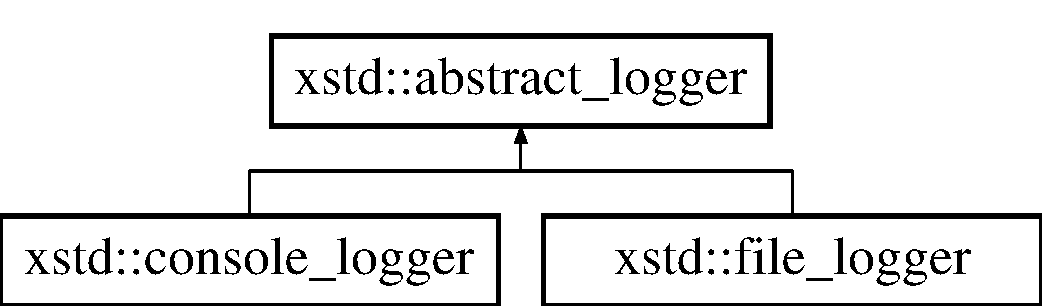
\includegraphics[height=2.000000cm]{classxstd_1_1abstract__logger}
\end{center}
\end{figure}
\subsection*{Public Member Functions}
\begin{DoxyCompactItemize}
\item 
\hypertarget{classxstd_1_1abstract__logger_a57d17bcf4d3260fab819d98643671c78}{{\bfseries abstract\-\_\-logger} (bool add\-\_\-new\-\_\-line=true, bool add\-\_\-time\-\_\-stamp=true) noexcept}\label{classxstd_1_1abstract__logger_a57d17bcf4d3260fab819d98643671c78}

\item 
\hypertarget{classxstd_1_1abstract__logger_ad470970ac4726355f3423017f434ace8}{void {\bfseries log} (const std\-::string \&data) const noexcept}\label{classxstd_1_1abstract__logger_ad470970ac4726355f3423017f434ace8}

\end{DoxyCompactItemize}
\subsection*{Public Attributes}
\begin{DoxyCompactItemize}
\item 
\hypertarget{classxstd_1_1abstract__logger_a5216ec0a18fea2571db19d5a55d8700f}{bool {\bfseries add\-\_\-new\-\_\-line}}\label{classxstd_1_1abstract__logger_a5216ec0a18fea2571db19d5a55d8700f}

\item 
\hypertarget{classxstd_1_1abstract__logger_a534b4f6a3dcdd3b7f18abfcb1bb5b937}{bool {\bfseries add\-\_\-time\-\_\-stamp}}\label{classxstd_1_1abstract__logger_a534b4f6a3dcdd3b7f18abfcb1bb5b937}

\end{DoxyCompactItemize}
\subsection*{Protected Member Functions}
\begin{DoxyCompactItemize}
\item 
\hypertarget{classxstd_1_1abstract__logger_a8cf4f5fd1490b54680060022a2f8ac91}{virtual void {\bfseries log\-\_\-data} (const std\-::string \&data) const noexcept=0}\label{classxstd_1_1abstract__logger_a8cf4f5fd1490b54680060022a2f8ac91}

\item 
\hypertarget{classxstd_1_1abstract__logger_a106b39652dd0d1efb32d8ad52ae6555c}{void {\bfseries log\-\_\-new\-\_\-line} (void) const noexcept}\label{classxstd_1_1abstract__logger_a106b39652dd0d1efb32d8ad52ae6555c}

\item 
\hypertarget{classxstd_1_1abstract__logger_a8bed4dfa79399f58146700adfd1ac06f}{void {\bfseries log\-\_\-time\-\_\-stamp} (void) const noexcept}\label{classxstd_1_1abstract__logger_a8bed4dfa79399f58146700adfd1ac06f}

\end{DoxyCompactItemize}
\subsection*{Static Protected Member Functions}
\begin{DoxyCompactItemize}
\item 
\hypertarget{classxstd_1_1abstract__logger_a1077a739173ed39b8f71f0ef69ada29f}{static std\-::string {\bfseries make\-\_\-time\-\_\-stamp} (void) noexcept}\label{classxstd_1_1abstract__logger_a1077a739173ed39b8f71f0ef69ada29f}

\end{DoxyCompactItemize}


The documentation for this class was generated from the following files\-:\begin{DoxyCompactItemize}
\item 
src/log/abstract\-\_\-logger/src/abstract\-\_\-logger.\-hpp\item 
src/log/abstract\-\_\-logger/src/abstract\-\_\-logger.\-ipp\end{DoxyCompactItemize}

\hypertarget{classxstd_1_1console__logger}{\section{xstd\-:\-:console\-\_\-logger Class Reference}
\label{classxstd_1_1console__logger}\index{xstd\-::console\-\_\-logger@{xstd\-::console\-\_\-logger}}
}


{\ttfamily \#include $<$console\-\_\-logger.\-hpp$>$}

Inheritance diagram for xstd\-:\-:console\-\_\-logger\-:\begin{figure}[H]
\begin{center}
\leavevmode
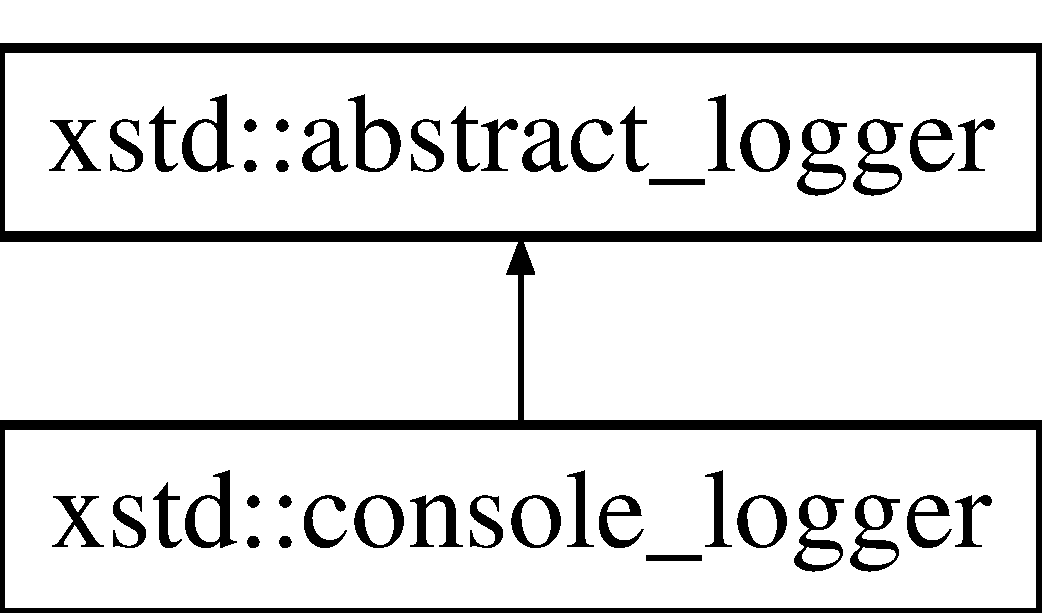
\includegraphics[height=2.000000cm]{classxstd_1_1console__logger}
\end{center}
\end{figure}
\subsection*{Public Member Functions}
\begin{DoxyCompactItemize}
\item 
\hyperlink{classxstd_1_1console__logger_a81ece8d9559e0ff0d54ad8d6cca596bc}{console\-\_\-logger} (bool \hyperlink{classxstd_1_1abstract__logger_a5216ec0a18fea2571db19d5a55d8700f}{add\-\_\-new\-\_\-line}=true, bool \hyperlink{classxstd_1_1abstract__logger_a534b4f6a3dcdd3b7f18abfcb1bb5b937}{add\-\_\-time\-\_\-stamp}=true) noexcept
\item 
void \hyperlink{classxstd_1_1abstract__logger_ad470970ac4726355f3423017f434ace8}{log} (const std\-::string \&data) const noexcept
\end{DoxyCompactItemize}
\subsection*{Public Attributes}
\begin{DoxyCompactItemize}
\item 
bool \hyperlink{classxstd_1_1abstract__logger_a5216ec0a18fea2571db19d5a55d8700f}{add\-\_\-new\-\_\-line}
\item 
bool \hyperlink{classxstd_1_1abstract__logger_a534b4f6a3dcdd3b7f18abfcb1bb5b937}{add\-\_\-time\-\_\-stamp}
\end{DoxyCompactItemize}
\subsection*{Protected Member Functions}
\begin{DoxyCompactItemize}
\item 
virtual void \hyperlink{classxstd_1_1console__logger_ad53afba0752b8cca7e5ccde101ec0954}{log\-\_\-data} (const std\-::string \&data) const noexcept override
\item 
void \hyperlink{classxstd_1_1abstract__logger_a106b39652dd0d1efb32d8ad52ae6555c}{log\-\_\-new\-\_\-line} (void) const noexcept
\item 
void \hyperlink{classxstd_1_1abstract__logger_a8bed4dfa79399f58146700adfd1ac06f}{log\-\_\-time\-\_\-stamp} (void) const noexcept
\end{DoxyCompactItemize}
\subsection*{Static Protected Member Functions}
\begin{DoxyCompactItemize}
\item 
static std\-::string \hyperlink{classxstd_1_1abstract__logger_a1077a739173ed39b8f71f0ef69ada29f}{make\-\_\-time\-\_\-stamp} (void) noexcept
\end{DoxyCompactItemize}


\subsection{Constructor \& Destructor Documentation}
\hypertarget{classxstd_1_1console__logger_a81ece8d9559e0ff0d54ad8d6cca596bc}{\index{xstd\-::console\-\_\-logger@{xstd\-::console\-\_\-logger}!console\-\_\-logger@{console\-\_\-logger}}
\index{console\-\_\-logger@{console\-\_\-logger}!xstd::console_logger@{xstd\-::console\-\_\-logger}}
\subsubsection[{console\-\_\-logger}]{\setlength{\rightskip}{0pt plus 5cm}xstd\-::console\-\_\-logger\-::console\-\_\-logger (
\begin{DoxyParamCaption}
\item[{bool}]{add\-\_\-new\-\_\-line = {\ttfamily true}, }
\item[{bool}]{add\-\_\-time\-\_\-stamp = {\ttfamily true}}
\end{DoxyParamCaption}
)\hspace{0.3cm}{\ttfamily [inline]}, {\ttfamily [explicit]}}}\label{classxstd_1_1console__logger_a81ece8d9559e0ff0d54ad8d6cca596bc}


\subsection{Member Function Documentation}
\hypertarget{classxstd_1_1abstract__logger_ad470970ac4726355f3423017f434ace8}{\index{xstd\-::console\-\_\-logger@{xstd\-::console\-\_\-logger}!log@{log}}
\index{log@{log}!xstd::console_logger@{xstd\-::console\-\_\-logger}}
\subsubsection[{log}]{\setlength{\rightskip}{0pt plus 5cm}void xstd\-::abstract\-\_\-logger\-::log (
\begin{DoxyParamCaption}
\item[{const std\-::string \&}]{data}
\end{DoxyParamCaption}
) const\hspace{0.3cm}{\ttfamily [inline]}, {\ttfamily [inherited]}}}\label{classxstd_1_1abstract__logger_ad470970ac4726355f3423017f434ace8}
\hypertarget{classxstd_1_1console__logger_ad53afba0752b8cca7e5ccde101ec0954}{\index{xstd\-::console\-\_\-logger@{xstd\-::console\-\_\-logger}!log\-\_\-data@{log\-\_\-data}}
\index{log\-\_\-data@{log\-\_\-data}!xstd::console_logger@{xstd\-::console\-\_\-logger}}
\subsubsection[{log\-\_\-data}]{\setlength{\rightskip}{0pt plus 5cm}void xstd\-::console\-\_\-logger\-::log\-\_\-data (
\begin{DoxyParamCaption}
\item[{const std\-::string \&}]{data}
\end{DoxyParamCaption}
) const\hspace{0.3cm}{\ttfamily [inline]}, {\ttfamily [override]}, {\ttfamily [protected]}, {\ttfamily [virtual]}}}\label{classxstd_1_1console__logger_ad53afba0752b8cca7e5ccde101ec0954}


Implements \hyperlink{classxstd_1_1abstract__logger_a8cf4f5fd1490b54680060022a2f8ac91}{xstd\-::abstract\-\_\-logger}.

\hypertarget{classxstd_1_1abstract__logger_a106b39652dd0d1efb32d8ad52ae6555c}{\index{xstd\-::console\-\_\-logger@{xstd\-::console\-\_\-logger}!log\-\_\-new\-\_\-line@{log\-\_\-new\-\_\-line}}
\index{log\-\_\-new\-\_\-line@{log\-\_\-new\-\_\-line}!xstd::console_logger@{xstd\-::console\-\_\-logger}}
\subsubsection[{log\-\_\-new\-\_\-line}]{\setlength{\rightskip}{0pt plus 5cm}void xstd\-::abstract\-\_\-logger\-::log\-\_\-new\-\_\-line (
\begin{DoxyParamCaption}
\item[{void}]{}
\end{DoxyParamCaption}
) const\hspace{0.3cm}{\ttfamily [inline]}, {\ttfamily [protected]}, {\ttfamily [inherited]}}}\label{classxstd_1_1abstract__logger_a106b39652dd0d1efb32d8ad52ae6555c}
\hypertarget{classxstd_1_1abstract__logger_a8bed4dfa79399f58146700adfd1ac06f}{\index{xstd\-::console\-\_\-logger@{xstd\-::console\-\_\-logger}!log\-\_\-time\-\_\-stamp@{log\-\_\-time\-\_\-stamp}}
\index{log\-\_\-time\-\_\-stamp@{log\-\_\-time\-\_\-stamp}!xstd::console_logger@{xstd\-::console\-\_\-logger}}
\subsubsection[{log\-\_\-time\-\_\-stamp}]{\setlength{\rightskip}{0pt plus 5cm}void xstd\-::abstract\-\_\-logger\-::log\-\_\-time\-\_\-stamp (
\begin{DoxyParamCaption}
\item[{void}]{}
\end{DoxyParamCaption}
) const\hspace{0.3cm}{\ttfamily [inline]}, {\ttfamily [protected]}, {\ttfamily [inherited]}}}\label{classxstd_1_1abstract__logger_a8bed4dfa79399f58146700adfd1ac06f}
\hypertarget{classxstd_1_1abstract__logger_a1077a739173ed39b8f71f0ef69ada29f}{\index{xstd\-::console\-\_\-logger@{xstd\-::console\-\_\-logger}!make\-\_\-time\-\_\-stamp@{make\-\_\-time\-\_\-stamp}}
\index{make\-\_\-time\-\_\-stamp@{make\-\_\-time\-\_\-stamp}!xstd::console_logger@{xstd\-::console\-\_\-logger}}
\subsubsection[{make\-\_\-time\-\_\-stamp}]{\setlength{\rightskip}{0pt plus 5cm}std\-::string xstd\-::abstract\-\_\-logger\-::make\-\_\-time\-\_\-stamp (
\begin{DoxyParamCaption}
\item[{void}]{}
\end{DoxyParamCaption}
)\hspace{0.3cm}{\ttfamily [inline]}, {\ttfamily [static]}, {\ttfamily [protected]}, {\ttfamily [inherited]}}}\label{classxstd_1_1abstract__logger_a1077a739173ed39b8f71f0ef69ada29f}


\subsection{Member Data Documentation}
\hypertarget{classxstd_1_1abstract__logger_a5216ec0a18fea2571db19d5a55d8700f}{\index{xstd\-::console\-\_\-logger@{xstd\-::console\-\_\-logger}!add\-\_\-new\-\_\-line@{add\-\_\-new\-\_\-line}}
\index{add\-\_\-new\-\_\-line@{add\-\_\-new\-\_\-line}!xstd::console_logger@{xstd\-::console\-\_\-logger}}
\subsubsection[{add\-\_\-new\-\_\-line}]{\setlength{\rightskip}{0pt plus 5cm}bool xstd\-::abstract\-\_\-logger\-::add\-\_\-new\-\_\-line\hspace{0.3cm}{\ttfamily [inherited]}}}\label{classxstd_1_1abstract__logger_a5216ec0a18fea2571db19d5a55d8700f}
\hypertarget{classxstd_1_1abstract__logger_a534b4f6a3dcdd3b7f18abfcb1bb5b937}{\index{xstd\-::console\-\_\-logger@{xstd\-::console\-\_\-logger}!add\-\_\-time\-\_\-stamp@{add\-\_\-time\-\_\-stamp}}
\index{add\-\_\-time\-\_\-stamp@{add\-\_\-time\-\_\-stamp}!xstd::console_logger@{xstd\-::console\-\_\-logger}}
\subsubsection[{add\-\_\-time\-\_\-stamp}]{\setlength{\rightskip}{0pt plus 5cm}bool xstd\-::abstract\-\_\-logger\-::add\-\_\-time\-\_\-stamp\hspace{0.3cm}{\ttfamily [inherited]}}}\label{classxstd_1_1abstract__logger_a534b4f6a3dcdd3b7f18abfcb1bb5b937}


The documentation for this class was generated from the following files\-:\begin{DoxyCompactItemize}
\item 
src/log/console\-\_\-logger/src/\hyperlink{console__logger_8hpp}{console\-\_\-logger.\-hpp}\item 
src/log/console\-\_\-logger/src/\hyperlink{console__logger_8ipp}{console\-\_\-logger.\-ipp}\end{DoxyCompactItemize}

\hypertarget{classxstd_1_1coutmt__singleton}{\section{xstd\-:\-:coutmt\-\_\-singleton Class Reference}
\label{classxstd_1_1coutmt__singleton}\index{xstd\-::coutmt\-\_\-singleton@{xstd\-::coutmt\-\_\-singleton}}
}
\subsection*{Static Public Member Functions}
\begin{DoxyCompactItemize}
\item 
\hypertarget{classxstd_1_1coutmt__singleton_a0c478170b82e253a79c51160fe7049a2}{static \hyperlink{classxstd_1_1coutmt__singleton}{coutmt\-\_\-singleton} \& {\bfseries get\-\_\-instance} (void)}\label{classxstd_1_1coutmt__singleton_a0c478170b82e253a79c51160fe7049a2}

\end{DoxyCompactItemize}
\subsection*{Friends}
\begin{DoxyCompactItemize}
\item 
\hypertarget{classxstd_1_1coutmt__singleton_aae5812b8fa2d66eaaa921e864e1077d4}{{\footnotesize template$<$typename Type $>$ }\\\hyperlink{classxstd_1_1coutmt__singleton}{coutmt\-\_\-singleton} \& {\bfseries operator$<$$<$} (\hyperlink{classxstd_1_1coutmt__singleton}{coutmt\-\_\-singleton} \&coutmt\-\_\-singleton\-\_\-instance, Type object)}\label{classxstd_1_1coutmt__singleton_aae5812b8fa2d66eaaa921e864e1077d4}

\item 
\hypertarget{classxstd_1_1coutmt__singleton_a75138493a4c47f61c28762df29d5af97}{\hyperlink{classxstd_1_1coutmt__singleton}{coutmt\-\_\-singleton} \& {\bfseries operator$<$$<$} (\hyperlink{classxstd_1_1coutmt__singleton}{coutmt\-\_\-singleton} \&coutmt\-\_\-singleton\-\_\-instance, std\-::ostream \&($\ast$function\-\_\-ptr)(std\-::ostream \&))}\label{classxstd_1_1coutmt__singleton_a75138493a4c47f61c28762df29d5af97}

\item 
\hypertarget{classxstd_1_1coutmt__singleton_af343264ff6f5ba75b8f6eab378c55638}{\hyperlink{classxstd_1_1coutmt__singleton}{coutmt\-\_\-singleton} \& {\bfseries operator$<$$<$} (\hyperlink{classxstd_1_1coutmt__singleton}{coutmt\-\_\-singleton} \&coutmt\-\_\-singleton\-\_\-instance, std\-::ios \&($\ast$function\-\_\-ptr)(std\-::ios \&))}\label{classxstd_1_1coutmt__singleton_af343264ff6f5ba75b8f6eab378c55638}

\item 
\hypertarget{classxstd_1_1coutmt__singleton_af794d8d7f2993af42e84429e5f5b4c9a}{\hyperlink{classxstd_1_1coutmt__singleton}{coutmt\-\_\-singleton} \& {\bfseries operator$<$$<$} (\hyperlink{classxstd_1_1coutmt__singleton}{coutmt\-\_\-singleton} \&coutmt\-\_\-singleton\-\_\-instance, std\-::ios\-\_\-base \&($\ast$function\-\_\-ptr)(std\-::ios\-\_\-base \&))}\label{classxstd_1_1coutmt__singleton_af794d8d7f2993af42e84429e5f5b4c9a}

\end{DoxyCompactItemize}


The documentation for this class was generated from the following files\-:\begin{DoxyCompactItemize}
\item 
src/iostream/coutmt/src/coutmt.\-hpp\item 
src/iostream/coutmt/src/coutmt.\-ipp\end{DoxyCompactItemize}

\hypertarget{structxstd_1_1dimension__mismatch}{\section{xstd\-:\-:dimension\-\_\-mismatch Struct Reference}
\label{structxstd_1_1dimension__mismatch}\index{xstd\-::dimension\-\_\-mismatch@{xstd\-::dimension\-\_\-mismatch}}
}


{\ttfamily \#include $<$point.\-hpp$>$}



The documentation for this struct was generated from the following file\-:\begin{DoxyCompactItemize}
\item 
src/cmath/point/src/\hyperlink{point_8hpp}{point.\-hpp}\end{DoxyCompactItemize}

\hypertarget{classxstd_1_1event}{\section{xstd\-:\-:event$<$ data\-\_\-type $>$ Class Template Reference}
\label{classxstd_1_1event}\index{xstd\-::event$<$ data\-\_\-type $>$@{xstd\-::event$<$ data\-\_\-type $>$}}
}


{\ttfamily \#include $<$event.\-hpp$>$}

\subsection*{Public Member Functions}
\begin{DoxyCompactItemize}
\item 
virtual \hyperlink{classxstd_1_1event_a5818ac871d63b38a5409eb3b153c3bef}{$\sim$event} (void) noexcept
\item 
unsigned int \hyperlink{classxstd_1_1event_af5ce6caa7da361833c3098686a28eb4a}{get\-\_\-listeners\-\_\-count} (void) const 
\item 
unsigned int \hyperlink{classxstd_1_1event_a91e77f734b2fe690615a9684446594a9}{get\-\_\-free\-\_\-listeners\-\_\-count} (void) const 
\item 
unsigned int \hyperlink{classxstd_1_1event_a6aec13f27635f3ad58435337f6063659}{get\-\_\-functor\-\_\-listeners\-\_\-count} (void) const 
\item 
bool \hyperlink{classxstd_1_1event_a28d29a9104d4e8c3986376b2ffca0a48}{has\-\_\-listener} (free\-\_\-listener free\-\_\-listener\-\_\-instance) const 
\item 
{\footnotesize template$<$typename object\-\_\-type $>$ }\\bool \hyperlink{classxstd_1_1event_acbfdc5b60687237a2b42bc6e7d00d4a4}{has\-\_\-listener} (object\-\_\-type $\ast$object\-\_\-ptr, void(object\-\_\-type\-::$\ast$method\-\_\-ptr)(data\-\_\-type...)) const 
\item 
void \hyperlink{classxstd_1_1event_a6d7320f608d4f7b072b62a5e66ea8d62}{add\-\_\-listener} (free\-\_\-listener free\-\_\-listener\-\_\-instance)
\item 
{\footnotesize template$<$typename object\-\_\-type $>$ }\\void \hyperlink{classxstd_1_1event_aa58880f86e0e2e5653df91692f221604}{add\-\_\-listener} (object\-\_\-type $\ast$object\-\_\-ptr, void(object\-\_\-type\-::$\ast$method\-\_\-ptr)(data\-\_\-type...))
\item 
void \hyperlink{classxstd_1_1event_a19e40e6d6af2d565ef741ecfbfb2fda7}{remove\-\_\-listener} (free\-\_\-listener free\-\_\-listener\-\_\-instance)
\item 
{\footnotesize template$<$typename object\-\_\-type $>$ }\\void \hyperlink{classxstd_1_1event_a2ecf3e9a39708db0c28281dbb32d12da}{remove\-\_\-listener} (object\-\_\-type $\ast$object\-\_\-ptr, void(object\-\_\-type\-::$\ast$method\-\_\-ptr)(data\-\_\-type...))
\item 
void \hyperlink{classxstd_1_1event_a60e1b1471f7c50f764fcb8388ca56b47}{dispatch} (data\-\_\-type...\-data) const 
\end{DoxyCompactItemize}
\subsection*{Protected Member Functions}
\begin{DoxyCompactItemize}
\item 
void \hyperlink{classxstd_1_1event_a3b2ec0fe63b51f0a785663ff1cbaf897}{check\-\_\-has\-\_\-listener} (free\-\_\-listener free\-\_\-listener\-\_\-instance) const 
\item 
{\footnotesize template$<$typename object\-\_\-type $>$ }\\void \hyperlink{classxstd_1_1event_a4c8f61670b0145de08594411dab17b49}{check\-\_\-has\-\_\-listener} (object\-\_\-type $\ast$object\-\_\-ptr, void(object\-\_\-type\-::$\ast$method\-\_\-ptr)(data\-\_\-type...)) const 
\item 
void \hyperlink{classxstd_1_1event_a8720bdcd9e0e8588eadbca2750f751e0}{check\-\_\-has\-\_\-no\-\_\-listener} (free\-\_\-listener free\-\_\-listener\-\_\-instance) const 
\item 
{\footnotesize template$<$typename object\-\_\-type $>$ }\\void \hyperlink{classxstd_1_1event_a38563e182cb13274550c790f6c2d48e1}{check\-\_\-has\-\_\-no\-\_\-listener} (object\-\_\-type $\ast$object\-\_\-ptr, void(object\-\_\-type\-::$\ast$method\-\_\-ptr)(data\-\_\-type...)) const 
\item 
free\-\_\-listeners\-\_\-collection\-\_\-itr \hyperlink{classxstd_1_1event_ac5c004598aa8803f901597ade5aec2c2}{get\-\_\-listener\-\_\-itr} (free\-\_\-listener free\-\_\-listener\-\_\-instance) const 
\item 
{\footnotesize template$<$typename object\-\_\-type $>$ }\\functor\-\_\-listeners\-\_\-collection\-\_\-itr \hyperlink{classxstd_1_1event_a56491edd13a1c81766c8c770464e992a}{get\-\_\-listener\-\_\-itr} (object\-\_\-type $\ast$object\-\_\-ptr, void(object\-\_\-type\-::$\ast$method\-\_\-ptr)(data\-\_\-type...)) const 
\item 
void \hyperlink{classxstd_1_1event_ac3a4cf6f6d139f3ab31cd3ca1ebb42e0}{dispatch\-\_\-free\-\_\-listeners} (data\-\_\-type...\-data) const 
\item 
void \hyperlink{classxstd_1_1event_a3c82e7e9e05c4c44e65b32db7090bd3c}{dispatch\-\_\-functor\-\_\-listeners} (data\-\_\-type...\-data) const 
\end{DoxyCompactItemize}
\subsection*{Protected Attributes}
\begin{DoxyCompactItemize}
\item 
free\-\_\-listeners\-\_\-collection \hyperlink{classxstd_1_1event_a045873dfdf4fe07af8421d81592d3275}{free\-\_\-listeners}
\item 
functor\-\_\-listeners\-\_\-collection \hyperlink{classxstd_1_1event_a3e4c0ca4abd96a0af619cdb96e3cfef2}{functor\-\_\-listeners}
\item 
std\-::recursive\-\_\-mutex \hyperlink{classxstd_1_1event_afaaee3e44989122c9e1db6f4d1547de8}{master\-\_\-mutex}
\end{DoxyCompactItemize}


\subsection{Constructor \& Destructor Documentation}
\hypertarget{classxstd_1_1event_a5818ac871d63b38a5409eb3b153c3bef}{\index{xstd\-::event@{xstd\-::event}!$\sim$event@{$\sim$event}}
\index{$\sim$event@{$\sim$event}!xstd::event@{xstd\-::event}}
\subsubsection[{$\sim$event}]{\setlength{\rightskip}{0pt plus 5cm}template$<$typename... data\-\_\-type$>$ virtual {\bf xstd\-::event}$<$ data\-\_\-type $>$\-::$\sim${\bf event} (
\begin{DoxyParamCaption}
\item[{void}]{}
\end{DoxyParamCaption}
)\hspace{0.3cm}{\ttfamily [inline]}, {\ttfamily [virtual]}}}\label{classxstd_1_1event_a5818ac871d63b38a5409eb3b153c3bef}


\subsection{Member Function Documentation}
\hypertarget{classxstd_1_1event_a6d7320f608d4f7b072b62a5e66ea8d62}{\index{xstd\-::event@{xstd\-::event}!add\-\_\-listener@{add\-\_\-listener}}
\index{add\-\_\-listener@{add\-\_\-listener}!xstd::event@{xstd\-::event}}
\subsubsection[{add\-\_\-listener}]{\setlength{\rightskip}{0pt plus 5cm}template$<$typename... data\-\_\-type$>$ void {\bf xstd\-::event}$<$ data\-\_\-type $>$\-::add\-\_\-listener (
\begin{DoxyParamCaption}
\item[{free\-\_\-listener}]{free\-\_\-listener\-\_\-instance}
\end{DoxyParamCaption}
)\hspace{0.3cm}{\ttfamily [inline]}}}\label{classxstd_1_1event_a6d7320f608d4f7b072b62a5e66ea8d62}
\hypertarget{classxstd_1_1event_aa58880f86e0e2e5653df91692f221604}{\index{xstd\-::event@{xstd\-::event}!add\-\_\-listener@{add\-\_\-listener}}
\index{add\-\_\-listener@{add\-\_\-listener}!xstd::event@{xstd\-::event}}
\subsubsection[{add\-\_\-listener}]{\setlength{\rightskip}{0pt plus 5cm}template$<$typename... data\-\_\-type$>$ template$<$typename object\-\_\-type $>$ void {\bf xstd\-::event}$<$ data\-\_\-type $>$\-::add\-\_\-listener (
\begin{DoxyParamCaption}
\item[{object\-\_\-type $\ast$}]{object\-\_\-ptr, }
\item[{void(object\-\_\-type\-::$\ast$)(data\-\_\-type...)}]{method\-\_\-ptr}
\end{DoxyParamCaption}
)\hspace{0.3cm}{\ttfamily [inline]}}}\label{classxstd_1_1event_aa58880f86e0e2e5653df91692f221604}
\hypertarget{classxstd_1_1event_a3b2ec0fe63b51f0a785663ff1cbaf897}{\index{xstd\-::event@{xstd\-::event}!check\-\_\-has\-\_\-listener@{check\-\_\-has\-\_\-listener}}
\index{check\-\_\-has\-\_\-listener@{check\-\_\-has\-\_\-listener}!xstd::event@{xstd\-::event}}
\subsubsection[{check\-\_\-has\-\_\-listener}]{\setlength{\rightskip}{0pt plus 5cm}template$<$typename... data\-\_\-type$>$ void {\bf xstd\-::event}$<$ data\-\_\-type $>$\-::check\-\_\-has\-\_\-listener (
\begin{DoxyParamCaption}
\item[{free\-\_\-listener}]{free\-\_\-listener\-\_\-instance}
\end{DoxyParamCaption}
) const\hspace{0.3cm}{\ttfamily [inline]}, {\ttfamily [protected]}}}\label{classxstd_1_1event_a3b2ec0fe63b51f0a785663ff1cbaf897}
\hypertarget{classxstd_1_1event_a4c8f61670b0145de08594411dab17b49}{\index{xstd\-::event@{xstd\-::event}!check\-\_\-has\-\_\-listener@{check\-\_\-has\-\_\-listener}}
\index{check\-\_\-has\-\_\-listener@{check\-\_\-has\-\_\-listener}!xstd::event@{xstd\-::event}}
\subsubsection[{check\-\_\-has\-\_\-listener}]{\setlength{\rightskip}{0pt plus 5cm}template$<$typename... data\-\_\-type$>$ template$<$typename object\-\_\-type $>$ void {\bf xstd\-::event}$<$ data\-\_\-type $>$\-::check\-\_\-has\-\_\-listener (
\begin{DoxyParamCaption}
\item[{object\-\_\-type $\ast$}]{object\-\_\-ptr, }
\item[{void(object\-\_\-type\-::$\ast$)(data\-\_\-type...)}]{method\-\_\-ptr}
\end{DoxyParamCaption}
) const\hspace{0.3cm}{\ttfamily [inline]}, {\ttfamily [protected]}}}\label{classxstd_1_1event_a4c8f61670b0145de08594411dab17b49}
\hypertarget{classxstd_1_1event_a8720bdcd9e0e8588eadbca2750f751e0}{\index{xstd\-::event@{xstd\-::event}!check\-\_\-has\-\_\-no\-\_\-listener@{check\-\_\-has\-\_\-no\-\_\-listener}}
\index{check\-\_\-has\-\_\-no\-\_\-listener@{check\-\_\-has\-\_\-no\-\_\-listener}!xstd::event@{xstd\-::event}}
\subsubsection[{check\-\_\-has\-\_\-no\-\_\-listener}]{\setlength{\rightskip}{0pt plus 5cm}template$<$typename... data\-\_\-type$>$ void {\bf xstd\-::event}$<$ data\-\_\-type $>$\-::check\-\_\-has\-\_\-no\-\_\-listener (
\begin{DoxyParamCaption}
\item[{free\-\_\-listener}]{free\-\_\-listener\-\_\-instance}
\end{DoxyParamCaption}
) const\hspace{0.3cm}{\ttfamily [inline]}, {\ttfamily [protected]}}}\label{classxstd_1_1event_a8720bdcd9e0e8588eadbca2750f751e0}
\hypertarget{classxstd_1_1event_a38563e182cb13274550c790f6c2d48e1}{\index{xstd\-::event@{xstd\-::event}!check\-\_\-has\-\_\-no\-\_\-listener@{check\-\_\-has\-\_\-no\-\_\-listener}}
\index{check\-\_\-has\-\_\-no\-\_\-listener@{check\-\_\-has\-\_\-no\-\_\-listener}!xstd::event@{xstd\-::event}}
\subsubsection[{check\-\_\-has\-\_\-no\-\_\-listener}]{\setlength{\rightskip}{0pt plus 5cm}template$<$typename... data\-\_\-type$>$ template$<$typename object\-\_\-type $>$ void {\bf xstd\-::event}$<$ data\-\_\-type $>$\-::check\-\_\-has\-\_\-no\-\_\-listener (
\begin{DoxyParamCaption}
\item[{object\-\_\-type $\ast$}]{object\-\_\-ptr, }
\item[{void(object\-\_\-type\-::$\ast$)(data\-\_\-type...)}]{method\-\_\-ptr}
\end{DoxyParamCaption}
) const\hspace{0.3cm}{\ttfamily [inline]}, {\ttfamily [protected]}}}\label{classxstd_1_1event_a38563e182cb13274550c790f6c2d48e1}
\hypertarget{classxstd_1_1event_a60e1b1471f7c50f764fcb8388ca56b47}{\index{xstd\-::event@{xstd\-::event}!dispatch@{dispatch}}
\index{dispatch@{dispatch}!xstd::event@{xstd\-::event}}
\subsubsection[{dispatch}]{\setlength{\rightskip}{0pt plus 5cm}template$<$typename... data\-\_\-type$>$ void {\bf xstd\-::event}$<$ data\-\_\-type $>$\-::dispatch (
\begin{DoxyParamCaption}
\item[{data\-\_\-type...}]{data}
\end{DoxyParamCaption}
) const\hspace{0.3cm}{\ttfamily [inline]}}}\label{classxstd_1_1event_a60e1b1471f7c50f764fcb8388ca56b47}
\hypertarget{classxstd_1_1event_ac3a4cf6f6d139f3ab31cd3ca1ebb42e0}{\index{xstd\-::event@{xstd\-::event}!dispatch\-\_\-free\-\_\-listeners@{dispatch\-\_\-free\-\_\-listeners}}
\index{dispatch\-\_\-free\-\_\-listeners@{dispatch\-\_\-free\-\_\-listeners}!xstd::event@{xstd\-::event}}
\subsubsection[{dispatch\-\_\-free\-\_\-listeners}]{\setlength{\rightskip}{0pt plus 5cm}template$<$typename... data\-\_\-type$>$ void {\bf xstd\-::event}$<$ data\-\_\-type $>$\-::dispatch\-\_\-free\-\_\-listeners (
\begin{DoxyParamCaption}
\item[{data\-\_\-type...}]{data}
\end{DoxyParamCaption}
) const\hspace{0.3cm}{\ttfamily [inline]}, {\ttfamily [protected]}}}\label{classxstd_1_1event_ac3a4cf6f6d139f3ab31cd3ca1ebb42e0}
\hypertarget{classxstd_1_1event_a3c82e7e9e05c4c44e65b32db7090bd3c}{\index{xstd\-::event@{xstd\-::event}!dispatch\-\_\-functor\-\_\-listeners@{dispatch\-\_\-functor\-\_\-listeners}}
\index{dispatch\-\_\-functor\-\_\-listeners@{dispatch\-\_\-functor\-\_\-listeners}!xstd::event@{xstd\-::event}}
\subsubsection[{dispatch\-\_\-functor\-\_\-listeners}]{\setlength{\rightskip}{0pt plus 5cm}template$<$typename... data\-\_\-type$>$ void {\bf xstd\-::event}$<$ data\-\_\-type $>$\-::dispatch\-\_\-functor\-\_\-listeners (
\begin{DoxyParamCaption}
\item[{data\-\_\-type...}]{data}
\end{DoxyParamCaption}
) const\hspace{0.3cm}{\ttfamily [inline]}, {\ttfamily [protected]}}}\label{classxstd_1_1event_a3c82e7e9e05c4c44e65b32db7090bd3c}
\hypertarget{classxstd_1_1event_a91e77f734b2fe690615a9684446594a9}{\index{xstd\-::event@{xstd\-::event}!get\-\_\-free\-\_\-listeners\-\_\-count@{get\-\_\-free\-\_\-listeners\-\_\-count}}
\index{get\-\_\-free\-\_\-listeners\-\_\-count@{get\-\_\-free\-\_\-listeners\-\_\-count}!xstd::event@{xstd\-::event}}
\subsubsection[{get\-\_\-free\-\_\-listeners\-\_\-count}]{\setlength{\rightskip}{0pt plus 5cm}template$<$typename... data\-\_\-type$>$ unsigned int {\bf xstd\-::event}$<$ data\-\_\-type $>$\-::get\-\_\-free\-\_\-listeners\-\_\-count (
\begin{DoxyParamCaption}
\item[{void}]{}
\end{DoxyParamCaption}
) const\hspace{0.3cm}{\ttfamily [inline]}}}\label{classxstd_1_1event_a91e77f734b2fe690615a9684446594a9}
\hypertarget{classxstd_1_1event_a6aec13f27635f3ad58435337f6063659}{\index{xstd\-::event@{xstd\-::event}!get\-\_\-functor\-\_\-listeners\-\_\-count@{get\-\_\-functor\-\_\-listeners\-\_\-count}}
\index{get\-\_\-functor\-\_\-listeners\-\_\-count@{get\-\_\-functor\-\_\-listeners\-\_\-count}!xstd::event@{xstd\-::event}}
\subsubsection[{get\-\_\-functor\-\_\-listeners\-\_\-count}]{\setlength{\rightskip}{0pt plus 5cm}template$<$typename... data\-\_\-type$>$ unsigned int {\bf xstd\-::event}$<$ data\-\_\-type $>$\-::get\-\_\-functor\-\_\-listeners\-\_\-count (
\begin{DoxyParamCaption}
\item[{void}]{}
\end{DoxyParamCaption}
) const\hspace{0.3cm}{\ttfamily [inline]}}}\label{classxstd_1_1event_a6aec13f27635f3ad58435337f6063659}
\hypertarget{classxstd_1_1event_ac5c004598aa8803f901597ade5aec2c2}{\index{xstd\-::event@{xstd\-::event}!get\-\_\-listener\-\_\-itr@{get\-\_\-listener\-\_\-itr}}
\index{get\-\_\-listener\-\_\-itr@{get\-\_\-listener\-\_\-itr}!xstd::event@{xstd\-::event}}
\subsubsection[{get\-\_\-listener\-\_\-itr}]{\setlength{\rightskip}{0pt plus 5cm}template$<$typename... data\-\_\-type$>$ free\-\_\-listeners\-\_\-collection\-\_\-itr {\bf xstd\-::event}$<$ data\-\_\-type $>$\-::get\-\_\-listener\-\_\-itr (
\begin{DoxyParamCaption}
\item[{free\-\_\-listener}]{free\-\_\-listener\-\_\-instance}
\end{DoxyParamCaption}
) const\hspace{0.3cm}{\ttfamily [inline]}, {\ttfamily [protected]}}}\label{classxstd_1_1event_ac5c004598aa8803f901597ade5aec2c2}
\hypertarget{classxstd_1_1event_a56491edd13a1c81766c8c770464e992a}{\index{xstd\-::event@{xstd\-::event}!get\-\_\-listener\-\_\-itr@{get\-\_\-listener\-\_\-itr}}
\index{get\-\_\-listener\-\_\-itr@{get\-\_\-listener\-\_\-itr}!xstd::event@{xstd\-::event}}
\subsubsection[{get\-\_\-listener\-\_\-itr}]{\setlength{\rightskip}{0pt plus 5cm}template$<$typename... data\-\_\-type$>$ template$<$typename object\-\_\-type $>$ functor\-\_\-listeners\-\_\-collection\-\_\-itr {\bf xstd\-::event}$<$ data\-\_\-type $>$\-::get\-\_\-listener\-\_\-itr (
\begin{DoxyParamCaption}
\item[{object\-\_\-type $\ast$}]{object\-\_\-ptr, }
\item[{void(object\-\_\-type\-::$\ast$)(data\-\_\-type...)}]{method\-\_\-ptr}
\end{DoxyParamCaption}
) const\hspace{0.3cm}{\ttfamily [inline]}, {\ttfamily [protected]}}}\label{classxstd_1_1event_a56491edd13a1c81766c8c770464e992a}
\hypertarget{classxstd_1_1event_af5ce6caa7da361833c3098686a28eb4a}{\index{xstd\-::event@{xstd\-::event}!get\-\_\-listeners\-\_\-count@{get\-\_\-listeners\-\_\-count}}
\index{get\-\_\-listeners\-\_\-count@{get\-\_\-listeners\-\_\-count}!xstd::event@{xstd\-::event}}
\subsubsection[{get\-\_\-listeners\-\_\-count}]{\setlength{\rightskip}{0pt plus 5cm}template$<$typename... data\-\_\-type$>$ unsigned int {\bf xstd\-::event}$<$ data\-\_\-type $>$\-::get\-\_\-listeners\-\_\-count (
\begin{DoxyParamCaption}
\item[{void}]{}
\end{DoxyParamCaption}
) const\hspace{0.3cm}{\ttfamily [inline]}}}\label{classxstd_1_1event_af5ce6caa7da361833c3098686a28eb4a}
\hypertarget{classxstd_1_1event_a28d29a9104d4e8c3986376b2ffca0a48}{\index{xstd\-::event@{xstd\-::event}!has\-\_\-listener@{has\-\_\-listener}}
\index{has\-\_\-listener@{has\-\_\-listener}!xstd::event@{xstd\-::event}}
\subsubsection[{has\-\_\-listener}]{\setlength{\rightskip}{0pt plus 5cm}template$<$typename... data\-\_\-type$>$ bool {\bf xstd\-::event}$<$ data\-\_\-type $>$\-::has\-\_\-listener (
\begin{DoxyParamCaption}
\item[{free\-\_\-listener}]{free\-\_\-listener\-\_\-instance}
\end{DoxyParamCaption}
) const\hspace{0.3cm}{\ttfamily [inline]}}}\label{classxstd_1_1event_a28d29a9104d4e8c3986376b2ffca0a48}
\hypertarget{classxstd_1_1event_acbfdc5b60687237a2b42bc6e7d00d4a4}{\index{xstd\-::event@{xstd\-::event}!has\-\_\-listener@{has\-\_\-listener}}
\index{has\-\_\-listener@{has\-\_\-listener}!xstd::event@{xstd\-::event}}
\subsubsection[{has\-\_\-listener}]{\setlength{\rightskip}{0pt plus 5cm}template$<$typename... data\-\_\-type$>$ template$<$typename object\-\_\-type $>$ bool {\bf xstd\-::event}$<$ data\-\_\-type $>$\-::has\-\_\-listener (
\begin{DoxyParamCaption}
\item[{object\-\_\-type $\ast$}]{object\-\_\-ptr, }
\item[{void(object\-\_\-type\-::$\ast$)(data\-\_\-type...)}]{method\-\_\-ptr}
\end{DoxyParamCaption}
) const\hspace{0.3cm}{\ttfamily [inline]}}}\label{classxstd_1_1event_acbfdc5b60687237a2b42bc6e7d00d4a4}
\hypertarget{classxstd_1_1event_a19e40e6d6af2d565ef741ecfbfb2fda7}{\index{xstd\-::event@{xstd\-::event}!remove\-\_\-listener@{remove\-\_\-listener}}
\index{remove\-\_\-listener@{remove\-\_\-listener}!xstd::event@{xstd\-::event}}
\subsubsection[{remove\-\_\-listener}]{\setlength{\rightskip}{0pt plus 5cm}template$<$typename... data\-\_\-type$>$ void {\bf xstd\-::event}$<$ data\-\_\-type $>$\-::remove\-\_\-listener (
\begin{DoxyParamCaption}
\item[{free\-\_\-listener}]{free\-\_\-listener\-\_\-instance}
\end{DoxyParamCaption}
)\hspace{0.3cm}{\ttfamily [inline]}}}\label{classxstd_1_1event_a19e40e6d6af2d565ef741ecfbfb2fda7}
\hypertarget{classxstd_1_1event_a2ecf3e9a39708db0c28281dbb32d12da}{\index{xstd\-::event@{xstd\-::event}!remove\-\_\-listener@{remove\-\_\-listener}}
\index{remove\-\_\-listener@{remove\-\_\-listener}!xstd::event@{xstd\-::event}}
\subsubsection[{remove\-\_\-listener}]{\setlength{\rightskip}{0pt plus 5cm}template$<$typename... data\-\_\-type$>$ template$<$typename object\-\_\-type $>$ void {\bf xstd\-::event}$<$ data\-\_\-type $>$\-::remove\-\_\-listener (
\begin{DoxyParamCaption}
\item[{object\-\_\-type $\ast$}]{object\-\_\-ptr, }
\item[{void(object\-\_\-type\-::$\ast$)(data\-\_\-type...)}]{method\-\_\-ptr}
\end{DoxyParamCaption}
)\hspace{0.3cm}{\ttfamily [inline]}}}\label{classxstd_1_1event_a2ecf3e9a39708db0c28281dbb32d12da}


\subsection{Member Data Documentation}
\hypertarget{classxstd_1_1event_a045873dfdf4fe07af8421d81592d3275}{\index{xstd\-::event@{xstd\-::event}!free\-\_\-listeners@{free\-\_\-listeners}}
\index{free\-\_\-listeners@{free\-\_\-listeners}!xstd::event@{xstd\-::event}}
\subsubsection[{free\-\_\-listeners}]{\setlength{\rightskip}{0pt plus 5cm}template$<$typename... data\-\_\-type$>$ free\-\_\-listeners\-\_\-collection {\bf xstd\-::event}$<$ data\-\_\-type $>$\-::free\-\_\-listeners\hspace{0.3cm}{\ttfamily [mutable]}, {\ttfamily [protected]}}}\label{classxstd_1_1event_a045873dfdf4fe07af8421d81592d3275}
\hypertarget{classxstd_1_1event_a3e4c0ca4abd96a0af619cdb96e3cfef2}{\index{xstd\-::event@{xstd\-::event}!functor\-\_\-listeners@{functor\-\_\-listeners}}
\index{functor\-\_\-listeners@{functor\-\_\-listeners}!xstd::event@{xstd\-::event}}
\subsubsection[{functor\-\_\-listeners}]{\setlength{\rightskip}{0pt plus 5cm}template$<$typename... data\-\_\-type$>$ functor\-\_\-listeners\-\_\-collection {\bf xstd\-::event}$<$ data\-\_\-type $>$\-::functor\-\_\-listeners\hspace{0.3cm}{\ttfamily [mutable]}, {\ttfamily [protected]}}}\label{classxstd_1_1event_a3e4c0ca4abd96a0af619cdb96e3cfef2}
\hypertarget{classxstd_1_1event_afaaee3e44989122c9e1db6f4d1547de8}{\index{xstd\-::event@{xstd\-::event}!master\-\_\-mutex@{master\-\_\-mutex}}
\index{master\-\_\-mutex@{master\-\_\-mutex}!xstd::event@{xstd\-::event}}
\subsubsection[{master\-\_\-mutex}]{\setlength{\rightskip}{0pt plus 5cm}template$<$typename... data\-\_\-type$>$ std\-::recursive\-\_\-mutex {\bf xstd\-::event}$<$ data\-\_\-type $>$\-::master\-\_\-mutex\hspace{0.3cm}{\ttfamily [mutable]}, {\ttfamily [protected]}}}\label{classxstd_1_1event_afaaee3e44989122c9e1db6f4d1547de8}


The documentation for this class was generated from the following file\-:\begin{DoxyCompactItemize}
\item 
src/event/event/src/\hyperlink{event_8hpp}{event.\-hpp}\end{DoxyCompactItemize}

\hypertarget{classxstd_1_1file__logger}{\section{xstd\-:\-:file\-\_\-logger Class Reference}
\label{classxstd_1_1file__logger}\index{xstd\-::file\-\_\-logger@{xstd\-::file\-\_\-logger}}
}


{\ttfamily \#include $<$file\-\_\-logger.\-hpp$>$}

Inheritance diagram for xstd\-:\-:file\-\_\-logger\-:\begin{figure}[H]
\begin{center}
\leavevmode
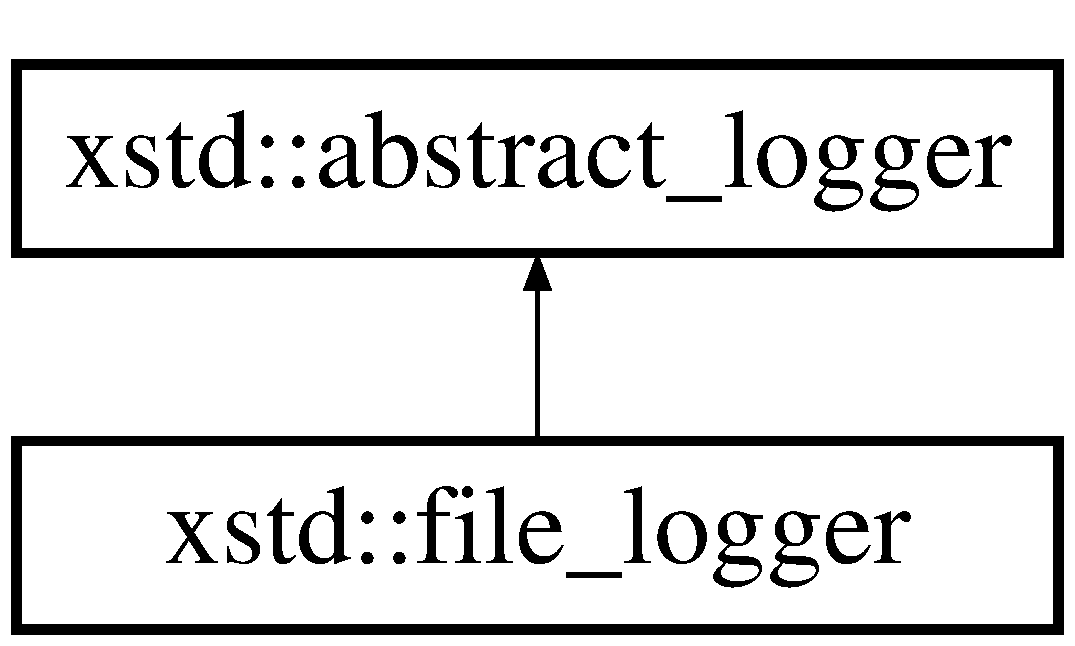
\includegraphics[height=2.000000cm]{classxstd_1_1file__logger}
\end{center}
\end{figure}
\subsection*{Public Member Functions}
\begin{DoxyCompactItemize}
\item 
\hyperlink{classxstd_1_1file__logger_a6e43dc8871b62e45550ce6470dcf5477}{file\-\_\-logger} (const std\-::string \&\hyperlink{classxstd_1_1file__logger_a0745eaab93df733f6696fa14e74eb068}{file}, bool \hyperlink{classxstd_1_1abstract__logger_a5216ec0a18fea2571db19d5a55d8700f}{add\-\_\-new\-\_\-line}=true, bool \hyperlink{classxstd_1_1abstract__logger_a534b4f6a3dcdd3b7f18abfcb1bb5b937}{add\-\_\-time\-\_\-stamp}=true) noexcept
\item 
void \hyperlink{classxstd_1_1abstract__logger_ad470970ac4726355f3423017f434ace8}{log} (const std\-::string \&data) const noexcept
\end{DoxyCompactItemize}
\subsection*{Public Attributes}
\begin{DoxyCompactItemize}
\item 
bool \hyperlink{classxstd_1_1abstract__logger_a5216ec0a18fea2571db19d5a55d8700f}{add\-\_\-new\-\_\-line}
\item 
bool \hyperlink{classxstd_1_1abstract__logger_a534b4f6a3dcdd3b7f18abfcb1bb5b937}{add\-\_\-time\-\_\-stamp}
\end{DoxyCompactItemize}
\subsection*{Protected Member Functions}
\begin{DoxyCompactItemize}
\item 
virtual void \hyperlink{classxstd_1_1file__logger_a806b0a7c20bad624afbddd2346312ca6}{log\-\_\-data} (const std\-::string \&data) const noexcept override
\item 
void \hyperlink{classxstd_1_1abstract__logger_a106b39652dd0d1efb32d8ad52ae6555c}{log\-\_\-new\-\_\-line} (void) const noexcept
\item 
void \hyperlink{classxstd_1_1abstract__logger_a8bed4dfa79399f58146700adfd1ac06f}{log\-\_\-time\-\_\-stamp} (void) const noexcept
\end{DoxyCompactItemize}
\subsection*{Static Protected Member Functions}
\begin{DoxyCompactItemize}
\item 
static std\-::string \hyperlink{classxstd_1_1abstract__logger_a1077a739173ed39b8f71f0ef69ada29f}{make\-\_\-time\-\_\-stamp} (void) noexcept
\end{DoxyCompactItemize}
\subsection*{Protected Attributes}
\begin{DoxyCompactItemize}
\item 
std\-::string \hyperlink{classxstd_1_1file__logger_a0745eaab93df733f6696fa14e74eb068}{file}
\end{DoxyCompactItemize}


\subsection{Constructor \& Destructor Documentation}
\hypertarget{classxstd_1_1file__logger_a6e43dc8871b62e45550ce6470dcf5477}{\index{xstd\-::file\-\_\-logger@{xstd\-::file\-\_\-logger}!file\-\_\-logger@{file\-\_\-logger}}
\index{file\-\_\-logger@{file\-\_\-logger}!xstd::file_logger@{xstd\-::file\-\_\-logger}}
\subsubsection[{file\-\_\-logger}]{\setlength{\rightskip}{0pt plus 5cm}xstd\-::file\-\_\-logger\-::file\-\_\-logger (
\begin{DoxyParamCaption}
\item[{const std\-::string \&}]{file, }
\item[{bool}]{add\-\_\-new\-\_\-line = {\ttfamily true}, }
\item[{bool}]{add\-\_\-time\-\_\-stamp = {\ttfamily true}}
\end{DoxyParamCaption}
)\hspace{0.3cm}{\ttfamily [inline]}, {\ttfamily [explicit]}}}\label{classxstd_1_1file__logger_a6e43dc8871b62e45550ce6470dcf5477}


\subsection{Member Function Documentation}
\hypertarget{classxstd_1_1abstract__logger_ad470970ac4726355f3423017f434ace8}{\index{xstd\-::file\-\_\-logger@{xstd\-::file\-\_\-logger}!log@{log}}
\index{log@{log}!xstd::file_logger@{xstd\-::file\-\_\-logger}}
\subsubsection[{log}]{\setlength{\rightskip}{0pt plus 5cm}void xstd\-::abstract\-\_\-logger\-::log (
\begin{DoxyParamCaption}
\item[{const std\-::string \&}]{data}
\end{DoxyParamCaption}
) const\hspace{0.3cm}{\ttfamily [inline]}, {\ttfamily [inherited]}}}\label{classxstd_1_1abstract__logger_ad470970ac4726355f3423017f434ace8}
\hypertarget{classxstd_1_1file__logger_a806b0a7c20bad624afbddd2346312ca6}{\index{xstd\-::file\-\_\-logger@{xstd\-::file\-\_\-logger}!log\-\_\-data@{log\-\_\-data}}
\index{log\-\_\-data@{log\-\_\-data}!xstd::file_logger@{xstd\-::file\-\_\-logger}}
\subsubsection[{log\-\_\-data}]{\setlength{\rightskip}{0pt plus 5cm}void xstd\-::file\-\_\-logger\-::log\-\_\-data (
\begin{DoxyParamCaption}
\item[{const std\-::string \&}]{data}
\end{DoxyParamCaption}
) const\hspace{0.3cm}{\ttfamily [inline]}, {\ttfamily [override]}, {\ttfamily [protected]}, {\ttfamily [virtual]}}}\label{classxstd_1_1file__logger_a806b0a7c20bad624afbddd2346312ca6}


Implements \hyperlink{classxstd_1_1abstract__logger_a8cf4f5fd1490b54680060022a2f8ac91}{xstd\-::abstract\-\_\-logger}.

\hypertarget{classxstd_1_1abstract__logger_a106b39652dd0d1efb32d8ad52ae6555c}{\index{xstd\-::file\-\_\-logger@{xstd\-::file\-\_\-logger}!log\-\_\-new\-\_\-line@{log\-\_\-new\-\_\-line}}
\index{log\-\_\-new\-\_\-line@{log\-\_\-new\-\_\-line}!xstd::file_logger@{xstd\-::file\-\_\-logger}}
\subsubsection[{log\-\_\-new\-\_\-line}]{\setlength{\rightskip}{0pt plus 5cm}void xstd\-::abstract\-\_\-logger\-::log\-\_\-new\-\_\-line (
\begin{DoxyParamCaption}
\item[{void}]{}
\end{DoxyParamCaption}
) const\hspace{0.3cm}{\ttfamily [inline]}, {\ttfamily [protected]}, {\ttfamily [inherited]}}}\label{classxstd_1_1abstract__logger_a106b39652dd0d1efb32d8ad52ae6555c}
\hypertarget{classxstd_1_1abstract__logger_a8bed4dfa79399f58146700adfd1ac06f}{\index{xstd\-::file\-\_\-logger@{xstd\-::file\-\_\-logger}!log\-\_\-time\-\_\-stamp@{log\-\_\-time\-\_\-stamp}}
\index{log\-\_\-time\-\_\-stamp@{log\-\_\-time\-\_\-stamp}!xstd::file_logger@{xstd\-::file\-\_\-logger}}
\subsubsection[{log\-\_\-time\-\_\-stamp}]{\setlength{\rightskip}{0pt plus 5cm}void xstd\-::abstract\-\_\-logger\-::log\-\_\-time\-\_\-stamp (
\begin{DoxyParamCaption}
\item[{void}]{}
\end{DoxyParamCaption}
) const\hspace{0.3cm}{\ttfamily [inline]}, {\ttfamily [protected]}, {\ttfamily [inherited]}}}\label{classxstd_1_1abstract__logger_a8bed4dfa79399f58146700adfd1ac06f}
\hypertarget{classxstd_1_1abstract__logger_a1077a739173ed39b8f71f0ef69ada29f}{\index{xstd\-::file\-\_\-logger@{xstd\-::file\-\_\-logger}!make\-\_\-time\-\_\-stamp@{make\-\_\-time\-\_\-stamp}}
\index{make\-\_\-time\-\_\-stamp@{make\-\_\-time\-\_\-stamp}!xstd::file_logger@{xstd\-::file\-\_\-logger}}
\subsubsection[{make\-\_\-time\-\_\-stamp}]{\setlength{\rightskip}{0pt plus 5cm}std\-::string xstd\-::abstract\-\_\-logger\-::make\-\_\-time\-\_\-stamp (
\begin{DoxyParamCaption}
\item[{void}]{}
\end{DoxyParamCaption}
)\hspace{0.3cm}{\ttfamily [inline]}, {\ttfamily [static]}, {\ttfamily [protected]}, {\ttfamily [inherited]}}}\label{classxstd_1_1abstract__logger_a1077a739173ed39b8f71f0ef69ada29f}


\subsection{Member Data Documentation}
\hypertarget{classxstd_1_1abstract__logger_a5216ec0a18fea2571db19d5a55d8700f}{\index{xstd\-::file\-\_\-logger@{xstd\-::file\-\_\-logger}!add\-\_\-new\-\_\-line@{add\-\_\-new\-\_\-line}}
\index{add\-\_\-new\-\_\-line@{add\-\_\-new\-\_\-line}!xstd::file_logger@{xstd\-::file\-\_\-logger}}
\subsubsection[{add\-\_\-new\-\_\-line}]{\setlength{\rightskip}{0pt plus 5cm}bool xstd\-::abstract\-\_\-logger\-::add\-\_\-new\-\_\-line\hspace{0.3cm}{\ttfamily [inherited]}}}\label{classxstd_1_1abstract__logger_a5216ec0a18fea2571db19d5a55d8700f}
\hypertarget{classxstd_1_1abstract__logger_a534b4f6a3dcdd3b7f18abfcb1bb5b937}{\index{xstd\-::file\-\_\-logger@{xstd\-::file\-\_\-logger}!add\-\_\-time\-\_\-stamp@{add\-\_\-time\-\_\-stamp}}
\index{add\-\_\-time\-\_\-stamp@{add\-\_\-time\-\_\-stamp}!xstd::file_logger@{xstd\-::file\-\_\-logger}}
\subsubsection[{add\-\_\-time\-\_\-stamp}]{\setlength{\rightskip}{0pt plus 5cm}bool xstd\-::abstract\-\_\-logger\-::add\-\_\-time\-\_\-stamp\hspace{0.3cm}{\ttfamily [inherited]}}}\label{classxstd_1_1abstract__logger_a534b4f6a3dcdd3b7f18abfcb1bb5b937}
\hypertarget{classxstd_1_1file__logger_a0745eaab93df733f6696fa14e74eb068}{\index{xstd\-::file\-\_\-logger@{xstd\-::file\-\_\-logger}!file@{file}}
\index{file@{file}!xstd::file_logger@{xstd\-::file\-\_\-logger}}
\subsubsection[{file}]{\setlength{\rightskip}{0pt plus 5cm}std\-::string xstd\-::file\-\_\-logger\-::file\hspace{0.3cm}{\ttfamily [protected]}}}\label{classxstd_1_1file__logger_a0745eaab93df733f6696fa14e74eb068}


The documentation for this class was generated from the following files\-:\begin{DoxyCompactItemize}
\item 
src/log/file\-\_\-logger/src/\hyperlink{file__logger_8hpp}{file\-\_\-logger.\-hpp}\item 
src/log/file\-\_\-logger/src/\hyperlink{file__logger_8ipp}{file\-\_\-logger.\-ipp}\end{DoxyCompactItemize}

\hypertarget{structxstd_1_1pp_1_1first__type}{\section{xstd\-:\-:pp\-:\-:first\-\_\-type$<$ parameters\-\_\-types $>$ Struct Template Reference}
\label{structxstd_1_1pp_1_1first__type}\index{xstd\-::pp\-::first\-\_\-type$<$ parameters\-\_\-types $>$@{xstd\-::pp\-::first\-\_\-type$<$ parameters\-\_\-types $>$}}
}


{\ttfamily \#include $<$parameter\-\_\-pack\-\_\-element\-\_\-type.\-hpp$>$}



The documentation for this struct was generated from the following file\-:\begin{DoxyCompactItemize}
\item 
src/utility/parameter\-\_\-pack/parameter\-\_\-pack\-\_\-element\-\_\-type/src/\hyperlink{parameter__pack__element__type_8hpp}{parameter\-\_\-pack\-\_\-element\-\_\-type.\-hpp}\end{DoxyCompactItemize}

\hypertarget{classxstd_1_1functor}{\section{xstd\-:\-:functor$<$ object\-\_\-type, arguments\-\_\-type $>$ Class Template Reference}
\label{classxstd_1_1functor}\index{xstd\-::functor$<$ object\-\_\-type, arguments\-\_\-type $>$@{xstd\-::functor$<$ object\-\_\-type, arguments\-\_\-type $>$}}
}
Inheritance diagram for xstd\-:\-:functor$<$ object\-\_\-type, arguments\-\_\-type $>$\-:\begin{figure}[H]
\begin{center}
\leavevmode
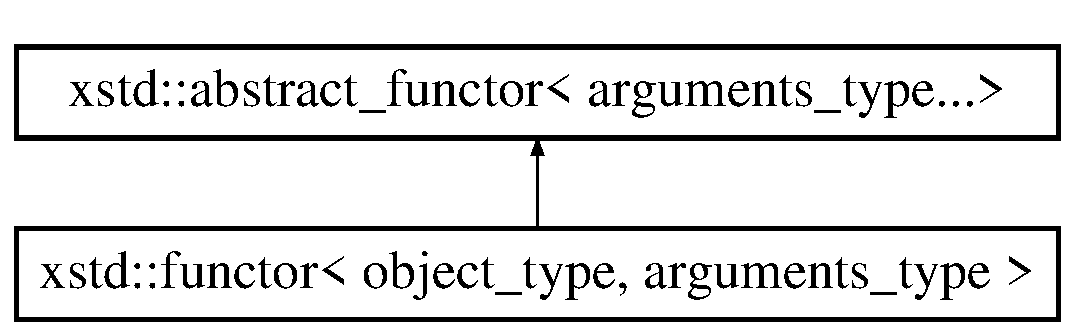
\includegraphics[height=2.000000cm]{classxstd_1_1functor}
\end{center}
\end{figure}
\subsection*{Public Member Functions}
\begin{DoxyCompactItemize}
\item 
\hypertarget{classxstd_1_1functor_aed2d510d4df5f6bb33d06370fbfa5fb8}{{\bfseries functor} (object\-\_\-type $\ast$object\-\_\-ptr, void(object\-\_\-type\-::$\ast$method\-\_\-ptr)(arguments\-\_\-type...))}\label{classxstd_1_1functor_aed2d510d4df5f6bb33d06370fbfa5fb8}

\item 
\hypertarget{classxstd_1_1functor_aeb8b8bd83b493e203d526dbf6b0c4920}{virtual void {\bfseries operator()} (arguments\-\_\-type...\-arguments) const override final}\label{classxstd_1_1functor_aeb8b8bd83b493e203d526dbf6b0c4920}

\item 
\hypertarget{classxstd_1_1functor_aa40709e615299c2c2d05c8c21c7ace66}{virtual void {\bfseries invoke} (arguments\-\_\-type...\-arguments) const override final}\label{classxstd_1_1functor_aa40709e615299c2c2d05c8c21c7ace66}

\end{DoxyCompactItemize}
\subsection*{Public Attributes}
\begin{DoxyCompactItemize}
\item 
\hypertarget{classxstd_1_1functor_a673d0ccf7da14d0d7f4726bbdf8af8a4}{void(object\-\_\-type\-::$\ast$ {\bfseries method\-\_\-ptr} )(arguments\-\_\-type...)}\label{classxstd_1_1functor_a673d0ccf7da14d0d7f4726bbdf8af8a4}

\item 
\hypertarget{classxstd_1_1functor_a919d42ea50702cf2ff02360f175b02ad}{object\-\_\-type $\ast$ {\bfseries object\-\_\-ptr}}\label{classxstd_1_1functor_a919d42ea50702cf2ff02360f175b02ad}

\end{DoxyCompactItemize}


The documentation for this class was generated from the following file\-:\begin{DoxyCompactItemize}
\item 
src/functional/functor/functor/src/functor.\-hpp\end{DoxyCompactItemize}

\hypertarget{structxstd_1_1pp_1_1is__heterogeneous}{\section{xstd\-:\-:pp\-:\-:is\-\_\-heterogeneous$<$ parameters\-\_\-types $>$ Struct Template Reference}
\label{structxstd_1_1pp_1_1is__heterogeneous}\index{xstd\-::pp\-::is\-\_\-heterogeneous$<$ parameters\-\_\-types $>$@{xstd\-::pp\-::is\-\_\-heterogeneous$<$ parameters\-\_\-types $>$}}
}


{\ttfamily \#include $<$parameter\-\_\-pack\-\_\-homogeneity.\-hpp$>$}

\subsection*{Static Public Attributes}
\begin{DoxyCompactItemize}
\item 
static const bool \hyperlink{structxstd_1_1pp_1_1is__heterogeneous_a790c8cb5a84cf3da91bf1602e181105b}{value} = ! \hyperlink{structxstd_1_1pp_1_1is__homogeneous}{is\-\_\-homogeneous}$<$parameters\-\_\-types...$>$\-::value
\end{DoxyCompactItemize}


\subsection{Member Data Documentation}
\hypertarget{structxstd_1_1pp_1_1is__heterogeneous_a790c8cb5a84cf3da91bf1602e181105b}{\index{xstd\-::pp\-::is\-\_\-heterogeneous@{xstd\-::pp\-::is\-\_\-heterogeneous}!value@{value}}
\index{value@{value}!xstd::pp::is_heterogeneous@{xstd\-::pp\-::is\-\_\-heterogeneous}}
\subsubsection[{value}]{\setlength{\rightskip}{0pt plus 5cm}template$<$typename... parameters\-\_\-types$>$ const bool {\bf xstd\-::pp\-::is\-\_\-heterogeneous}$<$ parameters\-\_\-types $>$\-::value = ! {\bf is\-\_\-homogeneous}$<$parameters\-\_\-types...$>$\-::value\hspace{0.3cm}{\ttfamily [static]}}}\label{structxstd_1_1pp_1_1is__heterogeneous_a790c8cb5a84cf3da91bf1602e181105b}


The documentation for this struct was generated from the following file\-:\begin{DoxyCompactItemize}
\item 
src/utility/parameter\-\_\-pack/parameter\-\_\-pack\-\_\-homogeneity/src/\hyperlink{parameter__pack__homogeneity_8hpp}{parameter\-\_\-pack\-\_\-homogeneity.\-hpp}\end{DoxyCompactItemize}

\hypertarget{structxstd_1_1pp_1_1is__homogeneous}{\section{xstd\-:\-:pp\-:\-:is\-\_\-homogeneous$<$ parameters\-\_\-types $>$ Struct Template Reference}
\label{structxstd_1_1pp_1_1is__homogeneous}\index{xstd\-::pp\-::is\-\_\-homogeneous$<$ parameters\-\_\-types $>$@{xstd\-::pp\-::is\-\_\-homogeneous$<$ parameters\-\_\-types $>$}}
}
\subsection*{Static Public Attributes}
\begin{DoxyCompactItemize}
\item 
\hypertarget{structxstd_1_1pp_1_1is__homogeneous_a104d1888e8f39e2d57ab27c7c3fb7383}{static const bool {\bfseries value} = true}\label{structxstd_1_1pp_1_1is__homogeneous_a104d1888e8f39e2d57ab27c7c3fb7383}

\end{DoxyCompactItemize}


The documentation for this struct was generated from the following file\-:\begin{DoxyCompactItemize}
\item 
src/utility/parameter\-\_\-pack/parameter\-\_\-pack\-\_\-homogeneity/src/parameter\-\_\-pack\-\_\-homogeneity.\-hpp\end{DoxyCompactItemize}

\hypertarget{structxstd_1_1pp_1_1is__homogeneous_3_01first__parameter__type_00_01other__parameters__types_8_8_8_01_4}{\section{xstd\-:\-:pp\-:\-:is\-\_\-homogeneous$<$ first\-\_\-parameter\-\_\-type, other\-\_\-parameters\-\_\-types... $>$ Struct Template Reference}
\label{structxstd_1_1pp_1_1is__homogeneous_3_01first__parameter__type_00_01other__parameters__types_8_8_8_01_4}\index{xstd\-::pp\-::is\-\_\-homogeneous$<$ first\-\_\-parameter\-\_\-type, other\-\_\-parameters\-\_\-types... $>$@{xstd\-::pp\-::is\-\_\-homogeneous$<$ first\-\_\-parameter\-\_\-type, other\-\_\-parameters\-\_\-types... $>$}}
}
\subsection*{Static Public Attributes}
\begin{DoxyCompactItemize}
\item 
\hypertarget{structxstd_1_1pp_1_1is__homogeneous_3_01first__parameter__type_00_01other__parameters__types_8_8_8_01_4_a7cb56d449b90e1ffbc9e9332d1faaa94}{static const bool {\bfseries value} = std\-::is\-\_\-same$<$first\-\_\-parameter\-\_\-type,other\-\_\-parameters\-\_\-type$>$\-::value}\label{structxstd_1_1pp_1_1is__homogeneous_3_01first__parameter__type_00_01other__parameters__types_8_8_8_01_4_a7cb56d449b90e1ffbc9e9332d1faaa94}

\end{DoxyCompactItemize}


The documentation for this struct was generated from the following file\-:\begin{DoxyCompactItemize}
\item 
src/utility/parameter\-\_\-pack/parameter\-\_\-pack\-\_\-homogeneity/src/parameter\-\_\-pack\-\_\-homogeneity.\-hpp\end{DoxyCompactItemize}

\hypertarget{structxstd_1_1pp_1_1is__homogeneous_3_01parameter__type_01_4}{\section{xstd\-:\-:pp\-:\-:is\-\_\-homogeneous$<$ parameter\-\_\-type $>$ Struct Template Reference}
\label{structxstd_1_1pp_1_1is__homogeneous_3_01parameter__type_01_4}\index{xstd\-::pp\-::is\-\_\-homogeneous$<$ parameter\-\_\-type $>$@{xstd\-::pp\-::is\-\_\-homogeneous$<$ parameter\-\_\-type $>$}}
}


{\ttfamily \#include $<$parameter\-\_\-pack\-\_\-homogeneity.\-hpp$>$}

\subsection*{Static Public Attributes}
\begin{DoxyCompactItemize}
\item 
static const bool \hyperlink{structxstd_1_1pp_1_1is__homogeneous_3_01parameter__type_01_4_a827e8f99e9ec9a203c3851ecd58dddb6}{value} = true
\end{DoxyCompactItemize}


\subsection{Member Data Documentation}
\hypertarget{structxstd_1_1pp_1_1is__homogeneous_3_01parameter__type_01_4_a827e8f99e9ec9a203c3851ecd58dddb6}{\index{xstd\-::pp\-::is\-\_\-homogeneous$<$ parameter\-\_\-type $>$@{xstd\-::pp\-::is\-\_\-homogeneous$<$ parameter\-\_\-type $>$}!value@{value}}
\index{value@{value}!xstd::pp::is_homogeneous< parameter_type >@{xstd\-::pp\-::is\-\_\-homogeneous$<$ parameter\-\_\-type $>$}}
\subsubsection[{value}]{\setlength{\rightskip}{0pt plus 5cm}template$<$typename parameter\-\_\-type $>$ const bool {\bf xstd\-::pp\-::is\-\_\-homogeneous}$<$ parameter\-\_\-type $>$\-::value = true\hspace{0.3cm}{\ttfamily [static]}}}\label{structxstd_1_1pp_1_1is__homogeneous_3_01parameter__type_01_4_a827e8f99e9ec9a203c3851ecd58dddb6}


The documentation for this struct was generated from the following file\-:\begin{DoxyCompactItemize}
\item 
src/utility/parameter\-\_\-pack/parameter\-\_\-pack\-\_\-homogeneity/src/\hyperlink{parameter__pack__homogeneity_8hpp}{parameter\-\_\-pack\-\_\-homogeneity.\-hpp}\end{DoxyCompactItemize}

\hypertarget{structxstd_1_1pp_1_1last__type}{\section{xstd\-:\-:pp\-:\-:last\-\_\-type$<$ parameters\-\_\-types $>$ Struct Template Reference}
\label{structxstd_1_1pp_1_1last__type}\index{xstd\-::pp\-::last\-\_\-type$<$ parameters\-\_\-types $>$@{xstd\-::pp\-::last\-\_\-type$<$ parameters\-\_\-types $>$}}
}


{\ttfamily \#include $<$parameter\-\_\-pack\-\_\-element\-\_\-type.\-hpp$>$}



The documentation for this struct was generated from the following file\-:\begin{DoxyCompactItemize}
\item 
src/utility/parameter\-\_\-pack/parameter\-\_\-pack\-\_\-element\-\_\-type/src/\hyperlink{parameter__pack__element__type_8hpp}{parameter\-\_\-pack\-\_\-element\-\_\-type.\-hpp}\end{DoxyCompactItemize}

\hypertarget{classxstd_1_1logger__client}{\section{xstd\-:\-:logger\-\_\-client Class Reference}
\label{classxstd_1_1logger__client}\index{xstd\-::logger\-\_\-client@{xstd\-::logger\-\_\-client}}
}
\subsection*{Public Member Functions}
\begin{DoxyCompactItemize}
\item 
\hypertarget{classxstd_1_1logger__client_ae366adb742d038fa072522500d798ce8}{{\bfseries logger\-\_\-client} (\hyperlink{classxstd_1_1abstract__logger}{abstract\-\_\-logger} $\ast$logger\-\_\-ptr=nullptr)}\label{classxstd_1_1logger__client_ae366adb742d038fa072522500d798ce8}

\item 
\hypertarget{classxstd_1_1logger__client_a4567aa30484c31b0d53089d1d08f8fab}{\hyperlink{classxstd_1_1abstract__logger}{abstract\-\_\-logger} \& {\bfseries get\-\_\-logger\-\_\-ref} (void)}\label{classxstd_1_1logger__client_a4567aa30484c31b0d53089d1d08f8fab}

\item 
\hypertarget{classxstd_1_1logger__client_a436c05e8f5d01fa5ed01aea36d1c5390}{\hyperlink{classxstd_1_1abstract__logger}{abstract\-\_\-logger} $\ast$ {\bfseries get\-\_\-logger\-\_\-ptr} (void)}\label{classxstd_1_1logger__client_a436c05e8f5d01fa5ed01aea36d1c5390}

\item 
\hypertarget{classxstd_1_1logger__client_a058f72e775905783e79721ecb2a65349}{void {\bfseries set\-\_\-logger} (\hyperlink{classxstd_1_1abstract__logger}{abstract\-\_\-logger} $\ast$logger\-\_\-ptr=nullptr)}\label{classxstd_1_1logger__client_a058f72e775905783e79721ecb2a65349}

\item 
\hypertarget{classxstd_1_1logger__client_a7169793d2c5512150d611ae47e0c6b74}{void {\bfseries log} (const std\-::string \&data) const }\label{classxstd_1_1logger__client_a7169793d2c5512150d611ae47e0c6b74}

\end{DoxyCompactItemize}
\subsection*{Protected Attributes}
\begin{DoxyCompactItemize}
\item 
\hypertarget{classxstd_1_1logger__client_a6f1cc6e74cfa370ec516e3fa792b3f1c}{\hyperlink{classxstd_1_1abstract__logger}{abstract\-\_\-logger} $\ast$ {\bfseries logger\-\_\-ptr}}\label{classxstd_1_1logger__client_a6f1cc6e74cfa370ec516e3fa792b3f1c}

\end{DoxyCompactItemize}


The documentation for this class was generated from the following files\-:\begin{DoxyCompactItemize}
\item 
src/log/logger\-\_\-client/src/logger\-\_\-client.\-hpp\item 
src/log/logger\-\_\-client/src/logger\-\_\-client.\-ipp\end{DoxyCompactItemize}

\hypertarget{structxstd_1_1pp_1_1nth__type}{\section{xstd\-:\-:pp\-:\-:nth\-\_\-type$<$ parameter\-\_\-id, parameters\-\_\-types $>$ Struct Template Reference}
\label{structxstd_1_1pp_1_1nth__type}\index{xstd\-::pp\-::nth\-\_\-type$<$ parameter\-\_\-id, parameters\-\_\-types $>$@{xstd\-::pp\-::nth\-\_\-type$<$ parameter\-\_\-id, parameters\-\_\-types $>$}}
}


{\ttfamily \#include $<$parameter\-\_\-pack\-\_\-element\-\_\-type.\-hpp$>$}



The documentation for this struct was generated from the following file\-:\begin{DoxyCompactItemize}
\item 
src/utility/parameter\-\_\-pack/parameter\-\_\-pack\-\_\-element\-\_\-type/src/\hyperlink{parameter__pack__element__type_8hpp}{parameter\-\_\-pack\-\_\-element\-\_\-type.\-hpp}\end{DoxyCompactItemize}

\hypertarget{structxstd_1_1pp_1_1nth__type__helper}{\section{xstd\-:\-:pp\-:\-:nth\-\_\-type\-\_\-helper$<$ parameter\-\_\-id, parameters\-\_\-types $>$ Struct Template Reference}
\label{structxstd_1_1pp_1_1nth__type__helper}\index{xstd\-::pp\-::nth\-\_\-type\-\_\-helper$<$ parameter\-\_\-id, parameters\-\_\-types $>$@{xstd\-::pp\-::nth\-\_\-type\-\_\-helper$<$ parameter\-\_\-id, parameters\-\_\-types $>$}}
}


{\ttfamily \#include $<$parameter\-\_\-pack\-\_\-element\-\_\-type.\-hpp$>$}



The documentation for this struct was generated from the following file\-:\begin{DoxyCompactItemize}
\item 
src/utility/parameter\-\_\-pack/parameter\-\_\-pack\-\_\-element\-\_\-type/src/\hyperlink{parameter__pack__element__type_8hpp}{parameter\-\_\-pack\-\_\-element\-\_\-type.\-hpp}\end{DoxyCompactItemize}

\hypertarget{structxstd_1_1pp_1_1nth__type__helper_3_010_00_01first__parameter__type_00_01other__parameters__types_8_8_8_01_4}{\section{xstd\-:\-:pp\-:\-:nth\-\_\-type\-\_\-helper$<$ 0, first\-\_\-parameter\-\_\-type, other\-\_\-parameters\-\_\-types... $>$ Struct Template Reference}
\label{structxstd_1_1pp_1_1nth__type__helper_3_010_00_01first__parameter__type_00_01other__parameters__types_8_8_8_01_4}\index{xstd\-::pp\-::nth\-\_\-type\-\_\-helper$<$ 0, first\-\_\-parameter\-\_\-type, other\-\_\-parameters\-\_\-types... $>$@{xstd\-::pp\-::nth\-\_\-type\-\_\-helper$<$ 0, first\-\_\-parameter\-\_\-type, other\-\_\-parameters\-\_\-types... $>$}}
}


The documentation for this struct was generated from the following file\-:\begin{DoxyCompactItemize}
\item 
src/utility/parameter\-\_\-pack/parameter\-\_\-pack\-\_\-element\-\_\-type/src/parameter\-\_\-pack\-\_\-element\-\_\-type.\-hpp\end{DoxyCompactItemize}

\hypertarget{structxstd_1_1pp_1_1nth__type__helper_3_01parameter__id_00_01first__parameter__type_00_01other__parameters__types_8_8_8_01_4}{\section{xstd\-:\-:pp\-:\-:nth\-\_\-type\-\_\-helper$<$ parameter\-\_\-id, first\-\_\-parameter\-\_\-type, other\-\_\-parameters\-\_\-types... $>$ Struct Template Reference}
\label{structxstd_1_1pp_1_1nth__type__helper_3_01parameter__id_00_01first__parameter__type_00_01other__parameters__types_8_8_8_01_4}\index{xstd\-::pp\-::nth\-\_\-type\-\_\-helper$<$ parameter\-\_\-id, first\-\_\-parameter\-\_\-type, other\-\_\-parameters\-\_\-types... $>$@{xstd\-::pp\-::nth\-\_\-type\-\_\-helper$<$ parameter\-\_\-id, first\-\_\-parameter\-\_\-type, other\-\_\-parameters\-\_\-types... $>$}}
}


The documentation for this struct was generated from the following file\-:\begin{DoxyCompactItemize}
\item 
src/utility/parameter\-\_\-pack/parameter\-\_\-pack\-\_\-element\-\_\-type/src/parameter\-\_\-pack\-\_\-element\-\_\-type.\-hpp\end{DoxyCompactItemize}

\hypertarget{structxstd_1_1pp_1_1null__type}{\section{xstd\-:\-:pp\-:\-:null\-\_\-type Struct Reference}
\label{structxstd_1_1pp_1_1null__type}\index{xstd\-::pp\-::null\-\_\-type@{xstd\-::pp\-::null\-\_\-type}}
}


{\ttfamily \#include $<$parameter\-\_\-pack\-\_\-element\-\_\-type.\-hpp$>$}

\subsection*{Public Member Functions}
\begin{DoxyCompactItemize}
\item 
bool \hyperlink{structxstd_1_1pp_1_1null__type_ab9e5487aa630bf4bfd0b01c28cc0415e}{operator==} (const \hyperlink{structxstd_1_1pp_1_1null__type}{null\-\_\-type}) const 
\item 
bool \hyperlink{structxstd_1_1pp_1_1null__type_ab290a23fbfc450daa1db57bfea446268}{operator!=} (const \hyperlink{structxstd_1_1pp_1_1null__type}{null\-\_\-type}) const 
\end{DoxyCompactItemize}


\subsection{Member Function Documentation}
\hypertarget{structxstd_1_1pp_1_1null__type_ab290a23fbfc450daa1db57bfea446268}{\index{xstd\-::pp\-::null\-\_\-type@{xstd\-::pp\-::null\-\_\-type}!operator!=@{operator!=}}
\index{operator!=@{operator!=}!xstd::pp::null_type@{xstd\-::pp\-::null\-\_\-type}}
\subsubsection[{operator!=}]{\setlength{\rightskip}{0pt plus 5cm}bool xstd\-::pp\-::null\-\_\-type\-::operator!= (
\begin{DoxyParamCaption}
\item[{const {\bf null\-\_\-type}}]{}
\end{DoxyParamCaption}
) const\hspace{0.3cm}{\ttfamily [inline]}}}\label{structxstd_1_1pp_1_1null__type_ab290a23fbfc450daa1db57bfea446268}
\hypertarget{structxstd_1_1pp_1_1null__type_ab9e5487aa630bf4bfd0b01c28cc0415e}{\index{xstd\-::pp\-::null\-\_\-type@{xstd\-::pp\-::null\-\_\-type}!operator==@{operator==}}
\index{operator==@{operator==}!xstd::pp::null_type@{xstd\-::pp\-::null\-\_\-type}}
\subsubsection[{operator==}]{\setlength{\rightskip}{0pt plus 5cm}bool xstd\-::pp\-::null\-\_\-type\-::operator== (
\begin{DoxyParamCaption}
\item[{const {\bf null\-\_\-type}}]{}
\end{DoxyParamCaption}
) const\hspace{0.3cm}{\ttfamily [inline]}}}\label{structxstd_1_1pp_1_1null__type_ab9e5487aa630bf4bfd0b01c28cc0415e}


The documentation for this struct was generated from the following file\-:\begin{DoxyCompactItemize}
\item 
src/utility/parameter\-\_\-pack/parameter\-\_\-pack\-\_\-element\-\_\-type/src/\hyperlink{parameter__pack__element__type_8hpp}{parameter\-\_\-pack\-\_\-element\-\_\-type.\-hpp}\end{DoxyCompactItemize}

\hypertarget{classxstd_1_1point}{\section{xstd\-:\-:point$<$ type, dimension $>$ Class Template Reference}
\label{classxstd_1_1point}\index{xstd\-::point$<$ type, dimension $>$@{xstd\-::point$<$ type, dimension $>$}}
}
\subsection*{Public Member Functions}
\begin{DoxyCompactItemize}
\item 
\hypertarget{classxstd_1_1point_a31b7e462164c6071b3847b0ad0604ef0}{{\bfseries point} (const coordinates\-\_\-initializer\-\_\-list \&coordinates\-\_\-object)}\label{classxstd_1_1point_a31b7e462164c6071b3847b0ad0604ef0}

\item 
\hypertarget{classxstd_1_1point_a3895117f5b9d43c53a8da93528aba6f5}{{\footnotesize template$<$typename \-\_\-type $>$ }\\{\bfseries point} (const \hyperlink{classxstd_1_1point}{point}$<$ \-\_\-type, dimension $>$ \&point\-\_\-object)}\label{classxstd_1_1point_a3895117f5b9d43c53a8da93528aba6f5}

\item 
\hypertarget{classxstd_1_1point_a67d8aba62c4ebe7cf114a276e30336f2}{{\footnotesize template$<$typename \-\_\-type $>$ }\\\hyperlink{classxstd_1_1point}{point} \& {\bfseries operator=} (const \hyperlink{classxstd_1_1point}{point}$<$ \-\_\-type, dimension $>$ \&point\-\_\-object)}\label{classxstd_1_1point_a67d8aba62c4ebe7cf114a276e30336f2}

\item 
\hypertarget{classxstd_1_1point_aaf46d8e0e0676b0fb5e8d86a7742e2a1}{type \& {\bfseries operator\mbox{[}$\,$\mbox{]}} (const int coordinate\-Id)}\label{classxstd_1_1point_aaf46d8e0e0676b0fb5e8d86a7742e2a1}

\item 
\hypertarget{classxstd_1_1point_a39217029d54ae1c115cc79db3edc1e48}{const type \& {\bfseries operator\mbox{[}$\,$\mbox{]}} (const int coordinate\-Id) const }\label{classxstd_1_1point_a39217029d54ae1c115cc79db3edc1e48}

\item 
\hypertarget{classxstd_1_1point_a2f98209745efac5775e14315b58d5a1d}{{\footnotesize template$<$typename \-\_\-type $>$ }\\bool {\bfseries operator==} (const \hyperlink{classxstd_1_1point}{point}$<$ \-\_\-type, dimension $>$ \&point\-\_\-object) const }\label{classxstd_1_1point_a2f98209745efac5775e14315b58d5a1d}

\item 
\hypertarget{classxstd_1_1point_a41ffcfd2fbb0420aceb7a3d81950e945}{{\footnotesize template$<$typename \-\_\-type $>$ }\\bool {\bfseries operator!=} (const \hyperlink{classxstd_1_1point}{point}$<$ \-\_\-type, dimension $>$ \&point\-\_\-object) const }\label{classxstd_1_1point_a41ffcfd2fbb0420aceb7a3d81950e945}

\item 
\hypertarget{classxstd_1_1point_aae13ce0401101be7b26121f8be146f4b}{{\footnotesize template$<$typename \-\_\-type $>$ }\\\hyperlink{classxstd_1_1point}{point} {\bfseries operator+} (const \hyperlink{classxstd_1_1point}{point}$<$ \-\_\-type, dimension $>$ \&point\-\_\-object) const }\label{classxstd_1_1point_aae13ce0401101be7b26121f8be146f4b}

\item 
\hypertarget{classxstd_1_1point_ad1af00d4517e769e7da57cd26732a6ab}{{\footnotesize template$<$typename \-\_\-type $>$ }\\\hyperlink{classxstd_1_1point}{point} {\bfseries operator-\/} (const \hyperlink{classxstd_1_1point}{point}$<$ \-\_\-type, dimension $>$ \&point\-\_\-object) const }\label{classxstd_1_1point_ad1af00d4517e769e7da57cd26732a6ab}

\item 
\hypertarget{classxstd_1_1point_ac777d5594b34c30fe27bcd549ef89be4}{\hyperlink{classxstd_1_1point}{point} {\bfseries operator$\ast$} (const float multiplier) const }\label{classxstd_1_1point_ac777d5594b34c30fe27bcd549ef89be4}

\item 
\hypertarget{classxstd_1_1point_aa96d22aaf0a1687325dadaa832740c3e}{\hyperlink{classxstd_1_1point}{point} {\bfseries operator/} (const float multiplier) const }\label{classxstd_1_1point_aa96d22aaf0a1687325dadaa832740c3e}

\item 
\hypertarget{classxstd_1_1point_a766d0887be589b7448696e0c0b00d557}{int {\bfseries get\-\_\-dimension} (void) const }\label{classxstd_1_1point_a766d0887be589b7448696e0c0b00d557}

\item 
\hypertarget{classxstd_1_1point_ae0363f79e01bb646555c51dfd99444ca}{type {\bfseries get\-\_\-coordinate\-\_\-value} (const int coordinate\-Id) const }\label{classxstd_1_1point_ae0363f79e01bb646555c51dfd99444ca}

\item 
\hypertarget{classxstd_1_1point_a812c6e9c6b5e329897fbab3ccce407e7}{coordinates \& {\bfseries get\-\_\-coordinates\-\_\-ref} (void)}\label{classxstd_1_1point_a812c6e9c6b5e329897fbab3ccce407e7}

\item 
\hypertarget{classxstd_1_1point_aa6910f3a870a3844003ed1fa77dab3b9}{const coordinates \& {\bfseries get\-\_\-coordinates\-\_\-ref} (void) const }\label{classxstd_1_1point_aa6910f3a870a3844003ed1fa77dab3b9}

\item 
\hypertarget{classxstd_1_1point_a1926a1a02d788b584e7e994edb956d61}{{\footnotesize template$<$typename \-\_\-type $>$ }\\float {\bfseries get\-\_\-distance\-\_\-to} (const \hyperlink{classxstd_1_1point}{point}$<$ \-\_\-type, dimension $>$ \&point\-\_\-object) const }\label{classxstd_1_1point_a1926a1a02d788b584e7e994edb956d61}

\item 
\hypertarget{classxstd_1_1point_a468d82213633b70cb8c01f97838e6d49}{{\footnotesize template$<$typename \-\_\-type $>$ }\\void {\bfseries set\-\_\-coordinates\-\_\-values} (const \-\_\-type \&coordinates\-Value)}\label{classxstd_1_1point_a468d82213633b70cb8c01f97838e6d49}

\item 
\hypertarget{classxstd_1_1point_a239dbdfe4d96a38b9eacd76e972897c4}{void {\bfseries set\-\_\-coordinates\-\_\-values} (const coordinates\-\_\-initializer\-\_\-list \&coordinates\-\_\-object)}\label{classxstd_1_1point_a239dbdfe4d96a38b9eacd76e972897c4}

\item 
\hypertarget{classxstd_1_1point_a16ea81630c6918bca7393e7ce46e1691}{{\footnotesize template$<$typename \-\_\-type $>$ }\\void {\bfseries set\-\_\-coordinates\-\_\-values} (const std\-::array$<$ \-\_\-type, dimension $>$ \&coordinates\-\_\-object)}\label{classxstd_1_1point_a16ea81630c6918bca7393e7ce46e1691}

\item 
\hypertarget{classxstd_1_1point_a5e32aa4388cfc0d9b9b3df56c5d8bd91}{void {\bfseries validate\-\_\-dimension\-\_\-match} (const coordinates\-\_\-initializer\-\_\-list \&coordinates\-\_\-object) const }\label{classxstd_1_1point_a5e32aa4388cfc0d9b9b3df56c5d8bd91}

\item 
\hypertarget{classxstd_1_1point_a15edf9d511dcd8d27c98e77b18033573}{{\footnotesize template$<$typename \-\_\-type , int \-\_\-dimension$>$ }\\void {\bfseries validate\-\_\-dimension\-\_\-match} (const \hyperlink{classxstd_1_1point}{point}$<$ \-\_\-type, \-\_\-dimension $>$ \&) const }\label{classxstd_1_1point_a15edf9d511dcd8d27c98e77b18033573}

\item 
\hypertarget{classxstd_1_1point_a9c83662efe0927f03cb9cb1cfab796cd}{void {\bfseries validate\-\_\-coordinate\-\_\-id} (const int coordinate\-Id) const }\label{classxstd_1_1point_a9c83662efe0927f03cb9cb1cfab796cd}

\item 
\hypertarget{classxstd_1_1point_a1d9e30c142c79d1c21bdb271c81dabb5}{void {\bfseries validate\-\_\-dimension} (void) const }\label{classxstd_1_1point_a1d9e30c142c79d1c21bdb271c81dabb5}

\end{DoxyCompactItemize}
\subsection*{Protected Attributes}
\begin{DoxyCompactItemize}
\item 
\hypertarget{classxstd_1_1point_a6ee0acdc7f3fdd004426279d0d7963e6}{coordinates {\bfseries coordinates\-\_\-object}}\label{classxstd_1_1point_a6ee0acdc7f3fdd004426279d0d7963e6}

\end{DoxyCompactItemize}
\subsection*{Friends}
\begin{DoxyCompactItemize}
\item 
\hypertarget{classxstd_1_1point_a26f9c85c349535d8d87c0b2b4dda134e}{std\-::ostream \& {\bfseries operator$<$$<$} (std\-::ostream \&output\-Stream, const \hyperlink{classxstd_1_1point}{point} \&point\-\_\-object)}\label{classxstd_1_1point_a26f9c85c349535d8d87c0b2b4dda134e}

\end{DoxyCompactItemize}


The documentation for this class was generated from the following file\-:\begin{DoxyCompactItemize}
\item 
src/cmath/point/src/point.\-hpp\end{DoxyCompactItemize}

\hypertarget{structprinter}{\section{printer Struct Reference}
\label{structprinter}\index{printer@{printer}}
}
\subsection*{Static Public Member Functions}
\begin{DoxyCompactItemize}
\item 
\hypertarget{structprinter_a65d06f6b703eabfd57600550b27ef2ff}{{\footnotesize template$<$typename type $>$ }\\static void {\bfseries process} (type object)}\label{structprinter_a65d06f6b703eabfd57600550b27ef2ff}

\end{DoxyCompactItemize}


The documentation for this struct was generated from the following file\-:\begin{DoxyCompactItemize}
\item 
src/utility/parameter\-\_\-pack/parameter\-\_\-pack\-\_\-for\-\_\-each/tests/src/parameter\-\_\-pack\-\_\-for\-\_\-each\-\_\-tests.\-cpp\end{DoxyCompactItemize}

\hypertarget{classxstd_1_1raii__thread}{\section{xstd\-:\-:raii\-\_\-thread Class Reference}
\label{classxstd_1_1raii__thread}\index{xstd\-::raii\-\_\-thread@{xstd\-::raii\-\_\-thread}}
}
Inheritance diagram for xstd\-:\-:raii\-\_\-thread\-:\begin{figure}[H]
\begin{center}
\leavevmode
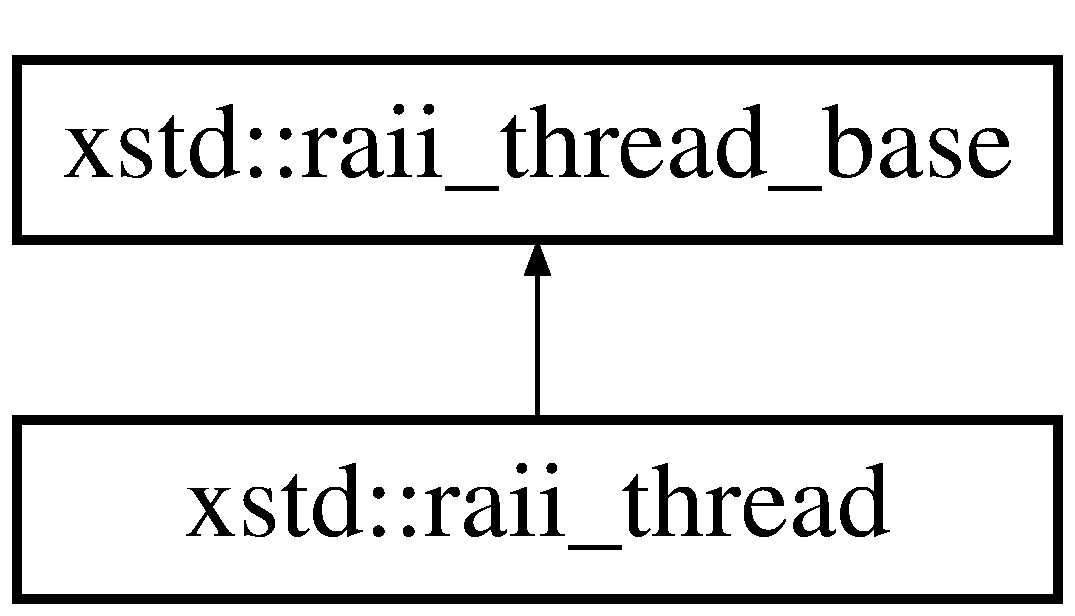
\includegraphics[height=2.000000cm]{classxstd_1_1raii__thread}
\end{center}
\end{figure}
\subsection*{Public Member Functions}
\begin{DoxyCompactItemize}
\item 
\hypertarget{classxstd_1_1raii__thread_a8bc39a85a55f9becb860febe87f9175c}{{\bfseries raii\-\_\-thread} (std\-::function$<$ void()$>$ client\-\_\-routine)}\label{classxstd_1_1raii__thread_a8bc39a85a55f9becb860febe87f9175c}

\end{DoxyCompactItemize}
\subsection*{Additional Inherited Members}


The documentation for this class was generated from the following files\-:\begin{DoxyCompactItemize}
\item 
src/thread/raii\-\_\-thread/src/raii\-\_\-thread.\-hpp\item 
src/thread/raii\-\_\-thread/src/raii\-\_\-thread.\-ipp\end{DoxyCompactItemize}

\hypertarget{classxstd_1_1raii__thread__base}{\section{xstd\-:\-:raii\-\_\-thread\-\_\-base Class Reference}
\label{classxstd_1_1raii__thread__base}\index{xstd\-::raii\-\_\-thread\-\_\-base@{xstd\-::raii\-\_\-thread\-\_\-base}}
}
Inheritance diagram for xstd\-:\-:raii\-\_\-thread\-\_\-base\-:\begin{figure}[H]
\begin{center}
\leavevmode
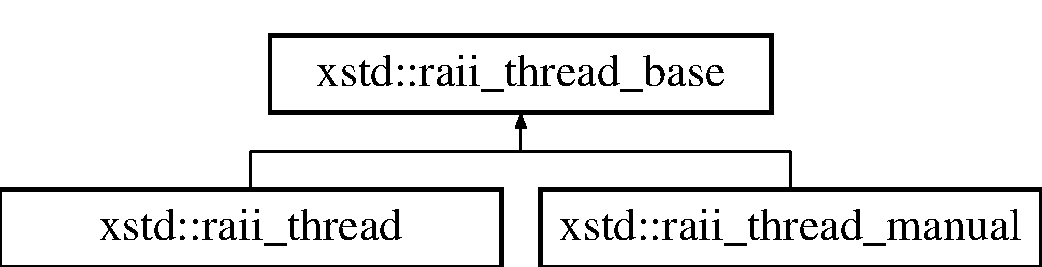
\includegraphics[height=2.000000cm]{classxstd_1_1raii__thread__base}
\end{center}
\end{figure}
\subsection*{Public Member Functions}
\begin{DoxyCompactItemize}
\item 
\hypertarget{classxstd_1_1raii__thread__base_a8f6cf744a47869c0e28a5e8a127c172b}{{\bfseries raii\-\_\-thread\-\_\-base} (std\-::function$<$ void()$>$ client\-\_\-routine)}\label{classxstd_1_1raii__thread__base_a8f6cf744a47869c0e28a5e8a127c172b}

\item 
\hypertarget{classxstd_1_1raii__thread__base_a9657cb2eddab6ef67b8884bff38ccbcb}{bool {\bfseries get\-\_\-is\-\_\-initialized} (void) const }\label{classxstd_1_1raii__thread__base_a9657cb2eddab6ef67b8884bff38ccbcb}

\end{DoxyCompactItemize}
\subsection*{Protected Member Functions}
\begin{DoxyCompactItemize}
\item 
\hypertarget{classxstd_1_1raii__thread__base_ad3b035606a096d6117de8de40c665507}{void {\bfseries initialize\-\_\-routine} (void)}\label{classxstd_1_1raii__thread__base_ad3b035606a096d6117de8de40c665507}

\item 
\hypertarget{classxstd_1_1raii__thread__base_ae423d8023eb8c3bed9b4b0f11c055c2d}{void {\bfseries deinitialize\-\_\-routine} (void)}\label{classxstd_1_1raii__thread__base_ae423d8023eb8c3bed9b4b0f11c055c2d}

\item 
\hypertarget{classxstd_1_1raii__thread__base_aef97fe42b58be66ddd0bf90462b772a8}{void {\bfseries check\-\_\-is\-\_\-initialized} (void) const }\label{classxstd_1_1raii__thread__base_aef97fe42b58be66ddd0bf90462b772a8}

\item 
\hypertarget{classxstd_1_1raii__thread__base_a6a179dd57da4ec48177c0cd38da0702e}{void {\bfseries check\-\_\-is\-\_\-not\-\_\-initialized} (void) const }\label{classxstd_1_1raii__thread__base_a6a179dd57da4ec48177c0cd38da0702e}

\end{DoxyCompactItemize}
\subsection*{Static Protected Member Functions}
\begin{DoxyCompactItemize}
\item 
\hypertarget{classxstd_1_1raii__thread__base_aac990e420873b2bb520e677156c37978}{static void {\bfseries routine} (\hyperlink{classxstd_1_1raii__thread__base}{raii\-\_\-thread\-\_\-base} $\ast$raii\-\_\-thread\-\_\-base\-\_\-ptr)}\label{classxstd_1_1raii__thread__base_aac990e420873b2bb520e677156c37978}

\end{DoxyCompactItemize}
\subsection*{Protected Attributes}
\begin{DoxyCompactItemize}
\item 
\hypertarget{classxstd_1_1raii__thread__base_aaac3bfb5572d71de17cb71d7ed0bb15c}{bool {\bfseries terminate\-\_\-flag}}\label{classxstd_1_1raii__thread__base_aaac3bfb5572d71de17cb71d7ed0bb15c}

\item 
\hypertarget{classxstd_1_1raii__thread__base_a6b3e160c7eb131008410a16c460b03ff}{std\-::function$<$ void()$>$ {\bfseries client\-\_\-routine}}\label{classxstd_1_1raii__thread__base_a6b3e160c7eb131008410a16c460b03ff}

\item 
\hypertarget{classxstd_1_1raii__thread__base_a664b3c47514557c3047e4ee0d7d9f25f}{std\-::thread {\bfseries thread}}\label{classxstd_1_1raii__thread__base_a664b3c47514557c3047e4ee0d7d9f25f}

\item 
\hypertarget{classxstd_1_1raii__thread__base_a9d9e01fced1a4f58ea5a9cc165f54fe3}{std\-::recursive\-\_\-mutex {\bfseries mutex}}\label{classxstd_1_1raii__thread__base_a9d9e01fced1a4f58ea5a9cc165f54fe3}

\end{DoxyCompactItemize}


The documentation for this class was generated from the following files\-:\begin{DoxyCompactItemize}
\item 
src/thread/raii\-\_\-thread\-\_\-base/src/raii\-\_\-thread\-\_\-base.\-hpp\item 
src/thread/raii\-\_\-thread\-\_\-base/src/raii\-\_\-thread\-\_\-base.\-ipp\end{DoxyCompactItemize}

\hypertarget{classxstd_1_1raii__thread__manual}{\section{xstd\-:\-:raii\-\_\-thread\-\_\-manual Class Reference}
\label{classxstd_1_1raii__thread__manual}\index{xstd\-::raii\-\_\-thread\-\_\-manual@{xstd\-::raii\-\_\-thread\-\_\-manual}}
}
Inheritance diagram for xstd\-:\-:raii\-\_\-thread\-\_\-manual\-:\begin{figure}[H]
\begin{center}
\leavevmode
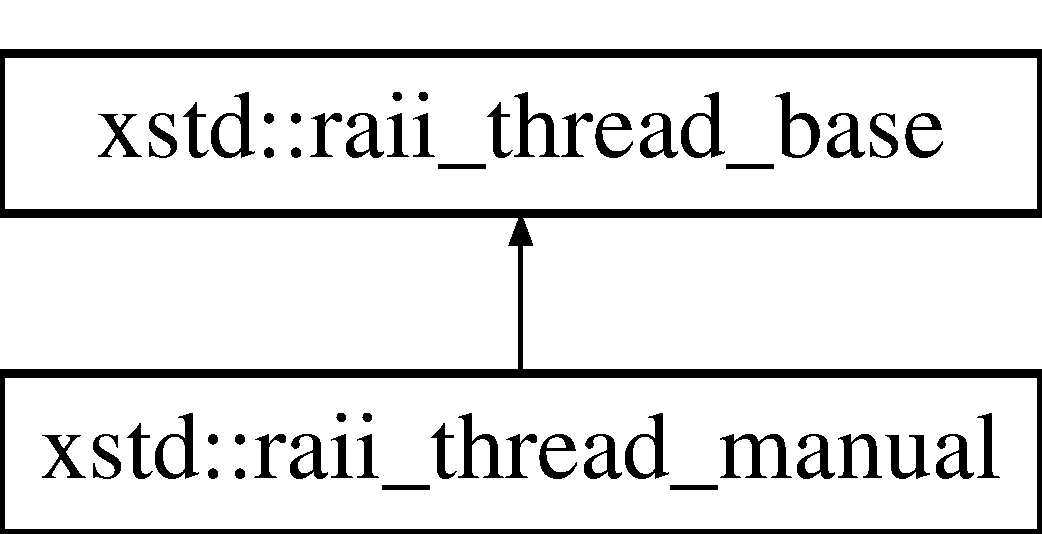
\includegraphics[height=2.000000cm]{classxstd_1_1raii__thread__manual}
\end{center}
\end{figure}
\subsection*{Public Member Functions}
\begin{DoxyCompactItemize}
\item 
\hypertarget{classxstd_1_1raii__thread__manual_a7a6c9e815d104ba820b3deaa5eef4000}{{\bfseries raii\-\_\-thread\-\_\-manual} (std\-::function$<$ void()$>$ client\-\_\-routine)}\label{classxstd_1_1raii__thread__manual_a7a6c9e815d104ba820b3deaa5eef4000}

\item 
\hypertarget{classxstd_1_1raii__thread__manual_a4998457f902ae8515ba0a37a8c78e37a}{void {\bfseries start} (void)}\label{classxstd_1_1raii__thread__manual_a4998457f902ae8515ba0a37a8c78e37a}

\item 
\hypertarget{classxstd_1_1raii__thread__manual_a00dc2a5fc7895b700a88afcdb9fa0f23}{void {\bfseries stop} (void)}\label{classxstd_1_1raii__thread__manual_a00dc2a5fc7895b700a88afcdb9fa0f23}

\end{DoxyCompactItemize}
\subsection*{Additional Inherited Members}


The documentation for this class was generated from the following files\-:\begin{DoxyCompactItemize}
\item 
src/thread/raii\-\_\-thread\-\_\-manual/src/raii\-\_\-thread\-\_\-manual.\-hpp\item 
src/thread/raii\-\_\-thread\-\_\-manual/src/raii\-\_\-thread\-\_\-manual.\-ipp\end{DoxyCompactItemize}

\hypertarget{classxstd_1_1chrono_1_1timer}{\section{xstd\-:\-:chrono\-:\-:timer$<$ clock $>$ Class Template Reference}
\label{classxstd_1_1chrono_1_1timer}\index{xstd\-::chrono\-::timer$<$ clock $>$@{xstd\-::chrono\-::timer$<$ clock $>$}}
}


{\ttfamily \#include $<$timer.\-hpp$>$}

Inheritance diagram for xstd\-:\-:chrono\-:\-:timer$<$ clock $>$\-:\begin{figure}[H]
\begin{center}
\leavevmode
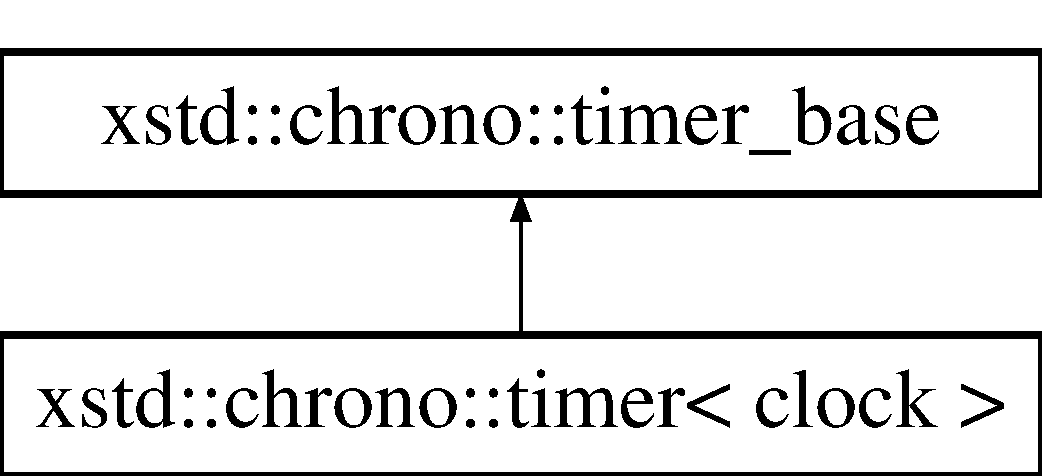
\includegraphics[height=2.000000cm]{classxstd_1_1chrono_1_1timer}
\end{center}
\end{figure}
\subsection*{Public Member Functions}
\begin{DoxyCompactItemize}
\item 
\hyperlink{classxstd_1_1chrono_1_1timer_a1d151d2452b9a4b5d00b37b238b86a9c}{timer} (void)
\item 
virtual \hyperlink{classxstd_1_1chrono_1_1timer_a274db25436fb2392246f64395ac4f2dc}{$\sim$timer} (void) noexcept
\item 
bool \hyperlink{classxstd_1_1chrono_1_1timer_a1496749b90d70cee8c29c66f9c67e21a}{get\-\_\-is\-\_\-active} (void) const 
\item 
void \hyperlink{classxstd_1_1chrono_1_1timer_a6ad3088df2f2ca33ea7246f1c716b65a}{get\-\_\-ticks\-\_\-done} (void) const 
\item 
void \hyperlink{classxstd_1_1chrono_1_1timer_a66a27994093e3a8cd5be70e82e577e25}{start} (void)
\item 
void \hyperlink{classxstd_1_1chrono_1_1timer_acb361a9fbbafe351513ee6251feb1000}{stop} (void)
\end{DoxyCompactItemize}
\subsection*{Public Attributes}
\begin{DoxyCompactItemize}
\item 
duration \hyperlink{classxstd_1_1chrono_1_1timer_a57838b4d220986131fcd8f5ddc1363bc}{tick\-\_\-interval}
\item 
unsigned int \hyperlink{classxstd_1_1chrono_1_1timer_a68ac37affa234daf952955ab2c1d674e}{tick\-\_\-limit}
\item 
event\-\_\-start\-\_\-type \hyperlink{classxstd_1_1chrono_1_1timer_acd6563ae4202b5d67856562d5a024894}{event\-\_\-start}
\item 
event\-\_\-tick\-\_\-type \hyperlink{classxstd_1_1chrono_1_1timer_a7bfca0bacd30aabd2bf7a69e25f2574c}{event\-\_\-tick}
\item 
event\-\_\-complete\-\_\-type \hyperlink{classxstd_1_1chrono_1_1timer_ac12f83ed705997b32c1dcf8853cf93c9}{event\-\_\-complete}
\item 
event\-\_\-stop\-\_\-type \hyperlink{classxstd_1_1chrono_1_1timer_a2f14e4ebe72f6c127f564f2dc4e97909}{event\-\_\-stop}
\end{DoxyCompactItemize}
\subsection*{Protected Member Functions}
\begin{DoxyCompactItemize}
\item 
bool \hyperlink{classxstd_1_1chrono_1_1timer_a79c070e4f1be92f8d8cf0cb62ebe0b2c}{requires\-\_\-tick} (void)
\item 
virtual void \hyperlink{classxstd_1_1chrono_1_1timer_a587e45f1e39ab87de14cda6f39e713da}{tick} (void) override
\item 
void \hyperlink{classxstd_1_1chrono_1_1timer_aef7b4094eebf22027987e81993859488}{update\-\_\-next\-\_\-tick\-\_\-time\-\_\-point} (void)
\item 
void \hyperlink{classxstd_1_1chrono_1_1timer_a6088ae4c5a93946c1159122305d76535}{check\-\_\-is\-\_\-ready\-\_\-to\-\_\-start} (void) const 
\item 
void \hyperlink{classxstd_1_1chrono_1_1timer_a631105f997839a66fb79c7ff87d83532}{check\-\_\-is\-\_\-ready\-\_\-to\-\_\-stop} (void) const 
\end{DoxyCompactItemize}
\subsection*{Protected Attributes}
\begin{DoxyCompactItemize}
\item 
bool \hyperlink{classxstd_1_1chrono_1_1timer_ac6a3c41d433b7e1387c297b925fb26d7}{is\-\_\-active}
\item 
unsigned int \hyperlink{classxstd_1_1chrono_1_1timer_a40ec5c890d4e54669729744b634daa9e}{ticks\-\_\-done}
\item 
time\-\_\-point \hyperlink{classxstd_1_1chrono_1_1timer_a51e85ae6c2a43cef074e5ff3e03620f9}{next\-\_\-tick\-\_\-time\-\_\-point}
\end{DoxyCompactItemize}


\subsection{Constructor \& Destructor Documentation}
\hypertarget{classxstd_1_1chrono_1_1timer_a1d151d2452b9a4b5d00b37b238b86a9c}{\index{xstd\-::chrono\-::timer@{xstd\-::chrono\-::timer}!timer@{timer}}
\index{timer@{timer}!xstd::chrono::timer@{xstd\-::chrono\-::timer}}
\subsubsection[{timer}]{\setlength{\rightskip}{0pt plus 5cm}template$<$typename clock  = std\-::chrono\-::high\-\_\-resolution\-\_\-clock$>$ {\bf xstd\-::chrono\-::timer}$<$ clock $>$\-::{\bf timer} (
\begin{DoxyParamCaption}
\item[{void}]{}
\end{DoxyParamCaption}
)\hspace{0.3cm}{\ttfamily [inline]}, {\ttfamily [explicit]}}}\label{classxstd_1_1chrono_1_1timer_a1d151d2452b9a4b5d00b37b238b86a9c}
\hypertarget{classxstd_1_1chrono_1_1timer_a274db25436fb2392246f64395ac4f2dc}{\index{xstd\-::chrono\-::timer@{xstd\-::chrono\-::timer}!$\sim$timer@{$\sim$timer}}
\index{$\sim$timer@{$\sim$timer}!xstd::chrono::timer@{xstd\-::chrono\-::timer}}
\subsubsection[{$\sim$timer}]{\setlength{\rightskip}{0pt plus 5cm}template$<$typename clock  = std\-::chrono\-::high\-\_\-resolution\-\_\-clock$>$ virtual {\bf xstd\-::chrono\-::timer}$<$ clock $>$\-::$\sim${\bf timer} (
\begin{DoxyParamCaption}
\item[{void}]{}
\end{DoxyParamCaption}
)\hspace{0.3cm}{\ttfamily [inline]}, {\ttfamily [virtual]}}}\label{classxstd_1_1chrono_1_1timer_a274db25436fb2392246f64395ac4f2dc}


\subsection{Member Function Documentation}
\hypertarget{classxstd_1_1chrono_1_1timer_a6088ae4c5a93946c1159122305d76535}{\index{xstd\-::chrono\-::timer@{xstd\-::chrono\-::timer}!check\-\_\-is\-\_\-ready\-\_\-to\-\_\-start@{check\-\_\-is\-\_\-ready\-\_\-to\-\_\-start}}
\index{check\-\_\-is\-\_\-ready\-\_\-to\-\_\-start@{check\-\_\-is\-\_\-ready\-\_\-to\-\_\-start}!xstd::chrono::timer@{xstd\-::chrono\-::timer}}
\subsubsection[{check\-\_\-is\-\_\-ready\-\_\-to\-\_\-start}]{\setlength{\rightskip}{0pt plus 5cm}template$<$typename clock  = std\-::chrono\-::high\-\_\-resolution\-\_\-clock$>$ void {\bf xstd\-::chrono\-::timer}$<$ clock $>$\-::check\-\_\-is\-\_\-ready\-\_\-to\-\_\-start (
\begin{DoxyParamCaption}
\item[{void}]{}
\end{DoxyParamCaption}
) const\hspace{0.3cm}{\ttfamily [inline]}, {\ttfamily [protected]}}}\label{classxstd_1_1chrono_1_1timer_a6088ae4c5a93946c1159122305d76535}
\hypertarget{classxstd_1_1chrono_1_1timer_a631105f997839a66fb79c7ff87d83532}{\index{xstd\-::chrono\-::timer@{xstd\-::chrono\-::timer}!check\-\_\-is\-\_\-ready\-\_\-to\-\_\-stop@{check\-\_\-is\-\_\-ready\-\_\-to\-\_\-stop}}
\index{check\-\_\-is\-\_\-ready\-\_\-to\-\_\-stop@{check\-\_\-is\-\_\-ready\-\_\-to\-\_\-stop}!xstd::chrono::timer@{xstd\-::chrono\-::timer}}
\subsubsection[{check\-\_\-is\-\_\-ready\-\_\-to\-\_\-stop}]{\setlength{\rightskip}{0pt plus 5cm}template$<$typename clock  = std\-::chrono\-::high\-\_\-resolution\-\_\-clock$>$ void {\bf xstd\-::chrono\-::timer}$<$ clock $>$\-::check\-\_\-is\-\_\-ready\-\_\-to\-\_\-stop (
\begin{DoxyParamCaption}
\item[{void}]{}
\end{DoxyParamCaption}
) const\hspace{0.3cm}{\ttfamily [inline]}, {\ttfamily [protected]}}}\label{classxstd_1_1chrono_1_1timer_a631105f997839a66fb79c7ff87d83532}
\hypertarget{classxstd_1_1chrono_1_1timer_a1496749b90d70cee8c29c66f9c67e21a}{\index{xstd\-::chrono\-::timer@{xstd\-::chrono\-::timer}!get\-\_\-is\-\_\-active@{get\-\_\-is\-\_\-active}}
\index{get\-\_\-is\-\_\-active@{get\-\_\-is\-\_\-active}!xstd::chrono::timer@{xstd\-::chrono\-::timer}}
\subsubsection[{get\-\_\-is\-\_\-active}]{\setlength{\rightskip}{0pt plus 5cm}template$<$typename clock  = std\-::chrono\-::high\-\_\-resolution\-\_\-clock$>$ bool {\bf xstd\-::chrono\-::timer}$<$ clock $>$\-::get\-\_\-is\-\_\-active (
\begin{DoxyParamCaption}
\item[{void}]{}
\end{DoxyParamCaption}
) const\hspace{0.3cm}{\ttfamily [inline]}}}\label{classxstd_1_1chrono_1_1timer_a1496749b90d70cee8c29c66f9c67e21a}
\hypertarget{classxstd_1_1chrono_1_1timer_a6ad3088df2f2ca33ea7246f1c716b65a}{\index{xstd\-::chrono\-::timer@{xstd\-::chrono\-::timer}!get\-\_\-ticks\-\_\-done@{get\-\_\-ticks\-\_\-done}}
\index{get\-\_\-ticks\-\_\-done@{get\-\_\-ticks\-\_\-done}!xstd::chrono::timer@{xstd\-::chrono\-::timer}}
\subsubsection[{get\-\_\-ticks\-\_\-done}]{\setlength{\rightskip}{0pt plus 5cm}template$<$typename clock  = std\-::chrono\-::high\-\_\-resolution\-\_\-clock$>$ void {\bf xstd\-::chrono\-::timer}$<$ clock $>$\-::get\-\_\-ticks\-\_\-done (
\begin{DoxyParamCaption}
\item[{void}]{}
\end{DoxyParamCaption}
) const\hspace{0.3cm}{\ttfamily [inline]}}}\label{classxstd_1_1chrono_1_1timer_a6ad3088df2f2ca33ea7246f1c716b65a}
\hypertarget{classxstd_1_1chrono_1_1timer_a79c070e4f1be92f8d8cf0cb62ebe0b2c}{\index{xstd\-::chrono\-::timer@{xstd\-::chrono\-::timer}!requires\-\_\-tick@{requires\-\_\-tick}}
\index{requires\-\_\-tick@{requires\-\_\-tick}!xstd::chrono::timer@{xstd\-::chrono\-::timer}}
\subsubsection[{requires\-\_\-tick}]{\setlength{\rightskip}{0pt plus 5cm}template$<$typename clock  = std\-::chrono\-::high\-\_\-resolution\-\_\-clock$>$ bool {\bf xstd\-::chrono\-::timer}$<$ clock $>$\-::requires\-\_\-tick (
\begin{DoxyParamCaption}
\item[{void}]{}
\end{DoxyParamCaption}
)\hspace{0.3cm}{\ttfamily [inline]}, {\ttfamily [protected]}}}\label{classxstd_1_1chrono_1_1timer_a79c070e4f1be92f8d8cf0cb62ebe0b2c}
\hypertarget{classxstd_1_1chrono_1_1timer_a66a27994093e3a8cd5be70e82e577e25}{\index{xstd\-::chrono\-::timer@{xstd\-::chrono\-::timer}!start@{start}}
\index{start@{start}!xstd::chrono::timer@{xstd\-::chrono\-::timer}}
\subsubsection[{start}]{\setlength{\rightskip}{0pt plus 5cm}template$<$typename clock  = std\-::chrono\-::high\-\_\-resolution\-\_\-clock$>$ void {\bf xstd\-::chrono\-::timer}$<$ clock $>$\-::start (
\begin{DoxyParamCaption}
\item[{void}]{}
\end{DoxyParamCaption}
)\hspace{0.3cm}{\ttfamily [inline]}}}\label{classxstd_1_1chrono_1_1timer_a66a27994093e3a8cd5be70e82e577e25}
\hypertarget{classxstd_1_1chrono_1_1timer_acb361a9fbbafe351513ee6251feb1000}{\index{xstd\-::chrono\-::timer@{xstd\-::chrono\-::timer}!stop@{stop}}
\index{stop@{stop}!xstd::chrono::timer@{xstd\-::chrono\-::timer}}
\subsubsection[{stop}]{\setlength{\rightskip}{0pt plus 5cm}template$<$typename clock  = std\-::chrono\-::high\-\_\-resolution\-\_\-clock$>$ void {\bf xstd\-::chrono\-::timer}$<$ clock $>$\-::stop (
\begin{DoxyParamCaption}
\item[{void}]{}
\end{DoxyParamCaption}
)\hspace{0.3cm}{\ttfamily [inline]}}}\label{classxstd_1_1chrono_1_1timer_acb361a9fbbafe351513ee6251feb1000}
\hypertarget{classxstd_1_1chrono_1_1timer_a587e45f1e39ab87de14cda6f39e713da}{\index{xstd\-::chrono\-::timer@{xstd\-::chrono\-::timer}!tick@{tick}}
\index{tick@{tick}!xstd::chrono::timer@{xstd\-::chrono\-::timer}}
\subsubsection[{tick}]{\setlength{\rightskip}{0pt plus 5cm}template$<$typename clock  = std\-::chrono\-::high\-\_\-resolution\-\_\-clock$>$ virtual void {\bf xstd\-::chrono\-::timer}$<$ clock $>$\-::tick (
\begin{DoxyParamCaption}
\item[{void}]{}
\end{DoxyParamCaption}
)\hspace{0.3cm}{\ttfamily [inline]}, {\ttfamily [override]}, {\ttfamily [protected]}, {\ttfamily [virtual]}}}\label{classxstd_1_1chrono_1_1timer_a587e45f1e39ab87de14cda6f39e713da}


Implements \hyperlink{classxstd_1_1chrono_1_1timer__base_a2d7c36af22ff593ca31849531fe23fd8}{xstd\-::chrono\-::timer\-\_\-base}.

\hypertarget{classxstd_1_1chrono_1_1timer_aef7b4094eebf22027987e81993859488}{\index{xstd\-::chrono\-::timer@{xstd\-::chrono\-::timer}!update\-\_\-next\-\_\-tick\-\_\-time\-\_\-point@{update\-\_\-next\-\_\-tick\-\_\-time\-\_\-point}}
\index{update\-\_\-next\-\_\-tick\-\_\-time\-\_\-point@{update\-\_\-next\-\_\-tick\-\_\-time\-\_\-point}!xstd::chrono::timer@{xstd\-::chrono\-::timer}}
\subsubsection[{update\-\_\-next\-\_\-tick\-\_\-time\-\_\-point}]{\setlength{\rightskip}{0pt plus 5cm}template$<$typename clock  = std\-::chrono\-::high\-\_\-resolution\-\_\-clock$>$ void {\bf xstd\-::chrono\-::timer}$<$ clock $>$\-::update\-\_\-next\-\_\-tick\-\_\-time\-\_\-point (
\begin{DoxyParamCaption}
\item[{void}]{}
\end{DoxyParamCaption}
)\hspace{0.3cm}{\ttfamily [inline]}, {\ttfamily [protected]}}}\label{classxstd_1_1chrono_1_1timer_aef7b4094eebf22027987e81993859488}


\subsection{Member Data Documentation}
\hypertarget{classxstd_1_1chrono_1_1timer_ac12f83ed705997b32c1dcf8853cf93c9}{\index{xstd\-::chrono\-::timer@{xstd\-::chrono\-::timer}!event\-\_\-complete@{event\-\_\-complete}}
\index{event\-\_\-complete@{event\-\_\-complete}!xstd::chrono::timer@{xstd\-::chrono\-::timer}}
\subsubsection[{event\-\_\-complete}]{\setlength{\rightskip}{0pt plus 5cm}template$<$typename clock  = std\-::chrono\-::high\-\_\-resolution\-\_\-clock$>$ event\-\_\-complete\-\_\-type {\bf xstd\-::chrono\-::timer}$<$ clock $>$\-::event\-\_\-complete}}\label{classxstd_1_1chrono_1_1timer_ac12f83ed705997b32c1dcf8853cf93c9}
\hypertarget{classxstd_1_1chrono_1_1timer_acd6563ae4202b5d67856562d5a024894}{\index{xstd\-::chrono\-::timer@{xstd\-::chrono\-::timer}!event\-\_\-start@{event\-\_\-start}}
\index{event\-\_\-start@{event\-\_\-start}!xstd::chrono::timer@{xstd\-::chrono\-::timer}}
\subsubsection[{event\-\_\-start}]{\setlength{\rightskip}{0pt plus 5cm}template$<$typename clock  = std\-::chrono\-::high\-\_\-resolution\-\_\-clock$>$ event\-\_\-start\-\_\-type {\bf xstd\-::chrono\-::timer}$<$ clock $>$\-::event\-\_\-start}}\label{classxstd_1_1chrono_1_1timer_acd6563ae4202b5d67856562d5a024894}
\hypertarget{classxstd_1_1chrono_1_1timer_a2f14e4ebe72f6c127f564f2dc4e97909}{\index{xstd\-::chrono\-::timer@{xstd\-::chrono\-::timer}!event\-\_\-stop@{event\-\_\-stop}}
\index{event\-\_\-stop@{event\-\_\-stop}!xstd::chrono::timer@{xstd\-::chrono\-::timer}}
\subsubsection[{event\-\_\-stop}]{\setlength{\rightskip}{0pt plus 5cm}template$<$typename clock  = std\-::chrono\-::high\-\_\-resolution\-\_\-clock$>$ event\-\_\-stop\-\_\-type {\bf xstd\-::chrono\-::timer}$<$ clock $>$\-::event\-\_\-stop}}\label{classxstd_1_1chrono_1_1timer_a2f14e4ebe72f6c127f564f2dc4e97909}
\hypertarget{classxstd_1_1chrono_1_1timer_a7bfca0bacd30aabd2bf7a69e25f2574c}{\index{xstd\-::chrono\-::timer@{xstd\-::chrono\-::timer}!event\-\_\-tick@{event\-\_\-tick}}
\index{event\-\_\-tick@{event\-\_\-tick}!xstd::chrono::timer@{xstd\-::chrono\-::timer}}
\subsubsection[{event\-\_\-tick}]{\setlength{\rightskip}{0pt plus 5cm}template$<$typename clock  = std\-::chrono\-::high\-\_\-resolution\-\_\-clock$>$ event\-\_\-tick\-\_\-type {\bf xstd\-::chrono\-::timer}$<$ clock $>$\-::event\-\_\-tick}}\label{classxstd_1_1chrono_1_1timer_a7bfca0bacd30aabd2bf7a69e25f2574c}
\hypertarget{classxstd_1_1chrono_1_1timer_ac6a3c41d433b7e1387c297b925fb26d7}{\index{xstd\-::chrono\-::timer@{xstd\-::chrono\-::timer}!is\-\_\-active@{is\-\_\-active}}
\index{is\-\_\-active@{is\-\_\-active}!xstd::chrono::timer@{xstd\-::chrono\-::timer}}
\subsubsection[{is\-\_\-active}]{\setlength{\rightskip}{0pt plus 5cm}template$<$typename clock  = std\-::chrono\-::high\-\_\-resolution\-\_\-clock$>$ bool {\bf xstd\-::chrono\-::timer}$<$ clock $>$\-::is\-\_\-active\hspace{0.3cm}{\ttfamily [protected]}}}\label{classxstd_1_1chrono_1_1timer_ac6a3c41d433b7e1387c297b925fb26d7}
\hypertarget{classxstd_1_1chrono_1_1timer_a51e85ae6c2a43cef074e5ff3e03620f9}{\index{xstd\-::chrono\-::timer@{xstd\-::chrono\-::timer}!next\-\_\-tick\-\_\-time\-\_\-point@{next\-\_\-tick\-\_\-time\-\_\-point}}
\index{next\-\_\-tick\-\_\-time\-\_\-point@{next\-\_\-tick\-\_\-time\-\_\-point}!xstd::chrono::timer@{xstd\-::chrono\-::timer}}
\subsubsection[{next\-\_\-tick\-\_\-time\-\_\-point}]{\setlength{\rightskip}{0pt plus 5cm}template$<$typename clock  = std\-::chrono\-::high\-\_\-resolution\-\_\-clock$>$ time\-\_\-point {\bf xstd\-::chrono\-::timer}$<$ clock $>$\-::next\-\_\-tick\-\_\-time\-\_\-point\hspace{0.3cm}{\ttfamily [protected]}}}\label{classxstd_1_1chrono_1_1timer_a51e85ae6c2a43cef074e5ff3e03620f9}
\hypertarget{classxstd_1_1chrono_1_1timer_a57838b4d220986131fcd8f5ddc1363bc}{\index{xstd\-::chrono\-::timer@{xstd\-::chrono\-::timer}!tick\-\_\-interval@{tick\-\_\-interval}}
\index{tick\-\_\-interval@{tick\-\_\-interval}!xstd::chrono::timer@{xstd\-::chrono\-::timer}}
\subsubsection[{tick\-\_\-interval}]{\setlength{\rightskip}{0pt plus 5cm}template$<$typename clock  = std\-::chrono\-::high\-\_\-resolution\-\_\-clock$>$ duration {\bf xstd\-::chrono\-::timer}$<$ clock $>$\-::tick\-\_\-interval}}\label{classxstd_1_1chrono_1_1timer_a57838b4d220986131fcd8f5ddc1363bc}
\hypertarget{classxstd_1_1chrono_1_1timer_a68ac37affa234daf952955ab2c1d674e}{\index{xstd\-::chrono\-::timer@{xstd\-::chrono\-::timer}!tick\-\_\-limit@{tick\-\_\-limit}}
\index{tick\-\_\-limit@{tick\-\_\-limit}!xstd::chrono::timer@{xstd\-::chrono\-::timer}}
\subsubsection[{tick\-\_\-limit}]{\setlength{\rightskip}{0pt plus 5cm}template$<$typename clock  = std\-::chrono\-::high\-\_\-resolution\-\_\-clock$>$ unsigned int {\bf xstd\-::chrono\-::timer}$<$ clock $>$\-::tick\-\_\-limit}}\label{classxstd_1_1chrono_1_1timer_a68ac37affa234daf952955ab2c1d674e}
\hypertarget{classxstd_1_1chrono_1_1timer_a40ec5c890d4e54669729744b634daa9e}{\index{xstd\-::chrono\-::timer@{xstd\-::chrono\-::timer}!ticks\-\_\-done@{ticks\-\_\-done}}
\index{ticks\-\_\-done@{ticks\-\_\-done}!xstd::chrono::timer@{xstd\-::chrono\-::timer}}
\subsubsection[{ticks\-\_\-done}]{\setlength{\rightskip}{0pt plus 5cm}template$<$typename clock  = std\-::chrono\-::high\-\_\-resolution\-\_\-clock$>$ unsigned int {\bf xstd\-::chrono\-::timer}$<$ clock $>$\-::ticks\-\_\-done\hspace{0.3cm}{\ttfamily [protected]}}}\label{classxstd_1_1chrono_1_1timer_a40ec5c890d4e54669729744b634daa9e}


The documentation for this class was generated from the following file\-:\begin{DoxyCompactItemize}
\item 
src/chrono/timer/timer/src/\hyperlink{timer_8hpp}{timer.\-hpp}\end{DoxyCompactItemize}

\hypertarget{classxstd_1_1chrono_1_1timer__base}{\section{xstd\-:\-:chrono\-:\-:timer\-\_\-base Class Reference}
\label{classxstd_1_1chrono_1_1timer__base}\index{xstd\-::chrono\-::timer\-\_\-base@{xstd\-::chrono\-::timer\-\_\-base}}
}
Inheritance diagram for xstd\-:\-:chrono\-:\-:timer\-\_\-base\-:\begin{figure}[H]
\begin{center}
\leavevmode
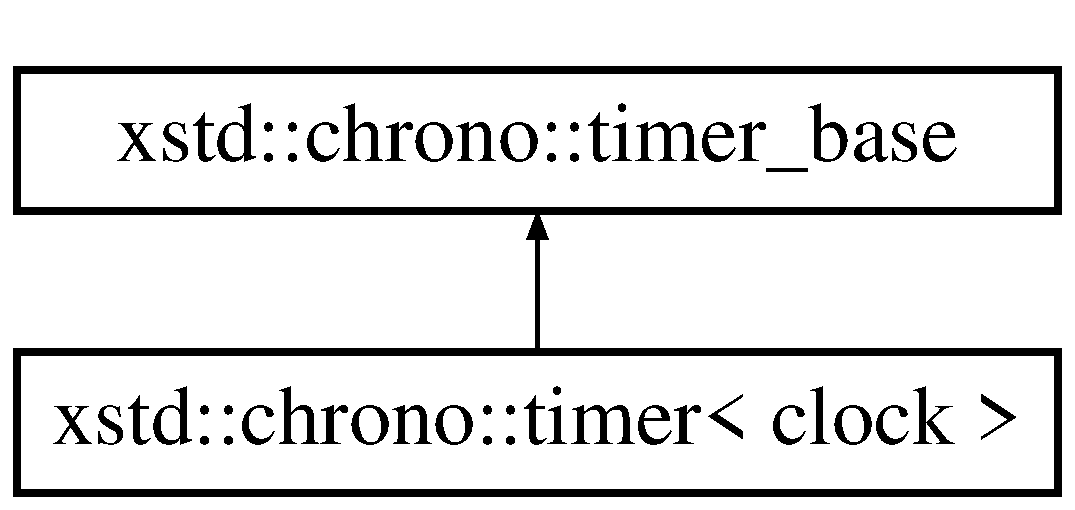
\includegraphics[height=2.000000cm]{classxstd_1_1chrono_1_1timer__base}
\end{center}
\end{figure}
\subsection*{Public Member Functions}
\begin{DoxyCompactItemize}
\item 
\hypertarget{classxstd_1_1chrono_1_1timer__base_a2d7c36af22ff593ca31849531fe23fd8}{virtual void {\bfseries tick} (void)=0}\label{classxstd_1_1chrono_1_1timer__base_a2d7c36af22ff593ca31849531fe23fd8}

\end{DoxyCompactItemize}


The documentation for this class was generated from the following file\-:\begin{DoxyCompactItemize}
\item 
src/chrono/timer/timer\-\_\-base/src/timer\-\_\-base.\-hpp\end{DoxyCompactItemize}

\hypertarget{classxstd_1_1chrono_1_1timer__manager}{\section{xstd\-:\-:chrono\-:\-:timer\-\_\-manager Class Reference}
\label{classxstd_1_1chrono_1_1timer__manager}\index{xstd\-::chrono\-::timer\-\_\-manager@{xstd\-::chrono\-::timer\-\_\-manager}}
}
\subsection*{Public Member Functions}
\begin{DoxyCompactItemize}
\item 
\hypertarget{classxstd_1_1chrono_1_1timer__manager_ae97c0dba8154bace5af93caae4948c8c}{void {\bfseries add\-\_\-timer} (\hyperlink{classxstd_1_1chrono_1_1timer__base}{timer\-\_\-base} $\ast$const timer\-\_\-ptr)}\label{classxstd_1_1chrono_1_1timer__manager_ae97c0dba8154bace5af93caae4948c8c}

\item 
\hypertarget{classxstd_1_1chrono_1_1timer__manager_af368bd572a757f8f78e39e4572114a84}{void {\bfseries remove\-\_\-timer} (\hyperlink{classxstd_1_1chrono_1_1timer__base}{timer\-\_\-base} $\ast$const timer\-\_\-ptr)}\label{classxstd_1_1chrono_1_1timer__manager_af368bd572a757f8f78e39e4572114a84}

\end{DoxyCompactItemize}
\subsection*{Static Public Member Functions}
\begin{DoxyCompactItemize}
\item 
\hypertarget{classxstd_1_1chrono_1_1timer__manager_a8894928f093db753153f2f87dfa511e0}{static \hyperlink{classxstd_1_1chrono_1_1timer__manager}{timer\-\_\-manager} \& {\bfseries get\-\_\-instance} (void)}\label{classxstd_1_1chrono_1_1timer__manager_a8894928f093db753153f2f87dfa511e0}

\end{DoxyCompactItemize}


The documentation for this class was generated from the following file\-:\begin{DoxyCompactItemize}
\item 
src/chrono/timer/timer\-\_\-manager/src/timer\-\_\-manager.\-hpp\end{DoxyCompactItemize}

\chapter{File Documentation}
\hypertarget{string__util_8hpp}{\section{src/string/string\-\_\-util/src/string\-\_\-util.hpp File Reference}
\label{string__util_8hpp}\index{src/string/string\-\_\-util/src/string\-\_\-util.\-hpp@{src/string/string\-\_\-util/src/string\-\_\-util.\-hpp}}
}
{\ttfamily \#include $<$stdexcept$>$}\\*
{\ttfamily \#include $<$algorithm$>$}\\*
{\ttfamily \#include $<$vector$>$}\\*
{\ttfamily \#include $<$sstream$>$}\\*
{\ttfamily \#include $<$climits$>$}\\*
{\ttfamily \#include $<$cstdlib$>$}\\*
{\ttfamily \#include \char`\"{}string\-\_\-util.\-ipp\char`\"{}}\\*
\subsection*{Namespaces}
\begin{DoxyCompactItemize}
\item 
namespace \hyperlink{namespacextd}{xtd}
\begin{DoxyCompactList}\small\item\em A root namespace of the library. \end{DoxyCompactList}\item 
namespace \hyperlink{namespacestr}{str}
\begin{DoxyCompactList}\small\item\em A namespace containing tools for operations which strings. \end{DoxyCompactList}\end{DoxyCompactItemize}
\subsection*{Functions}
\begin{DoxyCompactItemize}
\item 
signed long int {\bfseries xtd\-::str\-::string\-\_\-to\-\_\-long\-\_\-int} (const std\-::string \&source\-\_\-string, int number\-\_\-base=10)
\begin{DoxyCompactList}\small\item\em Converts a number from string to numeric representation. \end{DoxyCompactList}\item 
signed int {\bfseries xtd\-::str\-::string\-\_\-to\-\_\-int} (const std\-::string \&source\-\_\-string, int number\-\_\-base=10)
\begin{DoxyCompactList}\small\item\em Converts a number from string to numeric representation. \end{DoxyCompactList}\item 
\hypertarget{namespacextd_1_1str_aaabc2e3834d3052e392cda6140ae5cc2}{double {\bfseries xtd\-::str\-::string\-\_\-to\-\_\-double} (const std\-::string \&source\-\_\-string)}\label{namespacextd_1_1str_aaabc2e3834d3052e392cda6140ae5cc2}

\item 
\hypertarget{namespacextd_1_1str_a90f49ec1f4ff29fd05d598f815f9b4e0}{float {\bfseries xtd\-::str\-::string\-\_\-to\-\_\-float} (const std\-::string \&source\-\_\-string)}\label{namespacextd_1_1str_a90f49ec1f4ff29fd05d598f815f9b4e0}

\item 
\hypertarget{namespacextd_1_1str_a84c0f8285134f075fde7fbb91ee174ef}{std\-::string {\bfseries xtd\-::str\-::number\-\_\-to\-\_\-string} (int source\-\_\-number)}\label{namespacextd_1_1str_a84c0f8285134f075fde7fbb91ee174ef}

\item 
\hypertarget{namespacextd_1_1str_a485b63dcd6cac4d8b45712f634a2aaed}{std\-::string {\bfseries xtd\-::str\-::number\-\_\-to\-\_\-string} (unsigned int source\-\_\-number)}\label{namespacextd_1_1str_a485b63dcd6cac4d8b45712f634a2aaed}

\item 
\hypertarget{namespacextd_1_1str_ae520ea89838af34abca58612baf0ee7d}{std\-::string {\bfseries xtd\-::str\-::number\-\_\-to\-\_\-string} (float source\-\_\-number)}\label{namespacextd_1_1str_ae520ea89838af34abca58612baf0ee7d}

\item 
\hypertarget{namespacextd_1_1str_a0e5d3ce0842d8c4a0b42ec6bba6c5b00}{std\-::string {\bfseries xtd\-::str\-::string\-\_\-reverse} (const std\-::string \&source\-\_\-string)}\label{namespacextd_1_1str_a0e5d3ce0842d8c4a0b42ec6bba6c5b00}

\item 
\hypertarget{namespacextd_1_1str_a94ab05421170b46d98baffd7fbd04ae5}{strings {\bfseries xtd\-::str\-::string\-\_\-split} (const std\-::string \&source\-\_\-string, const std\-::string \&delimiter)}\label{namespacextd_1_1str_a94ab05421170b46d98baffd7fbd04ae5}

\item 
\hypertarget{namespacextd_1_1str_a06656216ad0df88bb608e00aaa18eb82}{strings {\bfseries xtd\-::str\-::string\-\_\-split} (const std\-::string \&source\-\_\-string, char delimiter)}\label{namespacextd_1_1str_a06656216ad0df88bb608e00aaa18eb82}

\item 
\hypertarget{namespacextd_1_1str_a1e141ef588bb3f2a3f586306377c0ad0}{strings {\bfseries xtd\-::str\-::string\-\_\-split} (const char $\ast$source\-\_\-string\-\_\-ptr, const char $\ast$delimiter\-\_\-ptr)}\label{namespacextd_1_1str_a1e141ef588bb3f2a3f586306377c0ad0}

\item 
\hypertarget{namespacextd_1_1str_a73aeee14b743df341c1b4a66199aa2c2}{std\-::string {\bfseries xtd\-::str\-::string\-\_\-replace} (const std\-::string \&source\-\_\-string, const std\-::string \&search\-\_\-for, const std\-::string \&replace\-\_\-with)}\label{namespacextd_1_1str_a73aeee14b743df341c1b4a66199aa2c2}

\item 
\hypertarget{namespacextd_1_1str_a76165b3eb4c578f41e935796ed4918c2}{std\-::string {\bfseries xtd\-::str\-::string\-\_\-replace} (const std\-::string \&source\-\_\-string, char search\-\_\-for, char replace\-\_\-with)}\label{namespacextd_1_1str_a76165b3eb4c578f41e935796ed4918c2}

\item 
\hypertarget{namespacextd_1_1str_a68fc51d9da10cd350332c3b29633088c}{std\-::string {\bfseries xtd\-::str\-::string\-\_\-replace} (const char $\ast$source\-\_\-string\-\_\-ptr, const char $\ast$search\-\_\-for\-\_\-ptr, const char $\ast$replace\-\_\-with\-\_\-ptr)}\label{namespacextd_1_1str_a68fc51d9da10cd350332c3b29633088c}

\item 
\hypertarget{namespacextd_1_1str_a6d1ae5acb732d24d3be7d1bc4baa7c47}{bool {\bfseries xtd\-::str\-::string\-\_\-is\-\_\-numeric} (const std\-::string \&source\-\_\-string)}\label{namespacextd_1_1str_a6d1ae5acb732d24d3be7d1bc4baa7c47}

\item 
\hypertarget{namespacextd_1_1str_a3b3cf2660283d567c5c46bafd478123e}{bool {\bfseries xtd\-::str\-::string\-\_\-is\-\_\-integer} (const std\-::string \&source\-\_\-string)}\label{namespacextd_1_1str_a3b3cf2660283d567c5c46bafd478123e}

\item 
\hypertarget{namespacextd_1_1str_a96ed87d80d055426e2a127049168552c}{bool {\bfseries xtd\-::str\-::string\-\_\-is\-\_\-fractional} (const std\-::string \&source\-\_\-string)}\label{namespacextd_1_1str_a96ed87d80d055426e2a127049168552c}

\end{DoxyCompactItemize}


\subsection{Detailed Description}

\printindex
\end{document}
